\documentclass[12pt,          % font size: 11pt or 12pt
               ms,           % degree:    ms or phd
               doublespacing % spacing: onehalfspacing or doublespacing
               ]{ncsuthesis}

%%----------------------------------------------------------------------------%%
%%------------------------------ Import Packages -----------------------------%%
%%----------------------------------------------------------------------------%%

\usepackage{booktabs}  % professionally typeset tables
\usepackage[fleqn]{amsmath}%,amssymb,amsfonts}
\usepackage{textcomp}  % better copyright sign, among other things
%\usepackage{xcolor}
\usepackage{subfig}    % composite figures
\usepackage[ruled,vlined,noresetcount ]{algorithm2e}
%%ORTIZ PACKAGES


%%%%%%%%%%%%%%%%%%%%%%%%%%%%%%%%%%%%%%%%%%
%%%%%%%%%%% Old bibliography commands
%%%%%%%%%%%%%%%%%%%%%%%%%%%%%%%%%%%%%%%%%%5
%\usepackage[super,sort&compress,comma,square,authoryear]{natbib} %\cite command %Added by Ortiz

%use the following line with plainnat
%\usepackage[super,sort&compress,comma,square,numbers]{natbib} %\cite command %Added by Ortiz
%\usepackage{natbib}

%\usepackage[style=alphabetic,natbib=true,backend=bibtex
%sorting=nyt,firstinits=true,isbn=false,doi=false,url=false]{biblatex} %couldn't get backend=biber to work

%\usepackage{filecontents}

%\bibliography{Ortiz-thesis2}
%\bibliographystyle{plain}


%%%%%%%%%%%%%%%%%%%%%%%%%%%%%%%%%%%%%%%%%%
%%%%%%%%%%% Hack for alphanumeric bibliography
%%%%%%%%%%%%%%%%%%%%%%%%%%%%%%%%%%%%%%%%%%5
\RequirePackage[
			style=numeric-comp,%alphabetic,%numeric-comp,%authoryear-comp,%
			sorting=nyt,%ynt					
			hyperref=true, %	
			firstinits=true,%
			backend=bibtex,
			natbib=true,
			url=false,
			isbn=false,
			maxnames=2, %for et al to be used
			maxalphanames=1, %to avoid printing a + for every et al in the abbreviation
			doi=false]{biblatex}		
			

%needed to do et al after two names
%http://tex.stackexchange.com/questions/44048/use-et-al-in-biblatex-custom-style
\renewcommand*{\finalnamedelim}{\addspace\&\space}

%Simplify abbreviation (the default uses either one or two authors and it indicates et al with a +)
%The following five lines make it so that only the first author is used in the abbreviation
%http://tex.stackexchange.com/questions/27956/label-only-from-first-author
\renewcommand*{\labelalphaothers}{}
    \renewcommand*{\intitlepunct}{}
    \DefineBibliographyStrings{german}{in={}}
    \DefineBibliographyStrings{english}{in={}}
    \DeclareNameAlias{sortname}{last-first}
    \DeclareNameAlias{default}{last-first}
	
%\AtEveryCitekey{\ifciteseen{}{\defcounter{maxnames}{99}}} %authoryear			
\DeclareFieldFormat[article,periodical]{volume}{\mkbibbold{#1}}
\makeatletter

\newrobustcmd*{\parentexttrack}[1]{%
  \begingroup
  \blx@blxinit
  \blx@setsfcodes
  \blx@bibopenparen#1\blx@bibcloseparen
  \endgroup}

\AtEveryCite{%
  \let\parentext=\parentexttrack%
  \let\bibopenparen=\bibopenbracket%
  \let\bibcloseparen=\bibclosebracket}

\makeatother
\renewcommand{\cite}[1]{\parencite{#1}}


\renewbibmacro{in:}{%
  \ifentrytype{article}{}{%
  \printtext{\bibstring{in}\intitlepunct}}}
  
\AtEveryBibitem{\clearfield{month}}

\AtEveryBibitem{\clearfield{language}}
%%%%%%%%%%%%%%%%%%%%%%%%%%%%%%%%%%%%%%%%%%%%%

%\addbibresource{Ortiz-thesis2.bib}
%\addbibresource{Ortiz-thesisURL.bib}
\addbibresource{PriteshRanjanThesis.bib}

 \defbibheading{myheading}[REFERENCES]{
 \chapter*{#1}
 %\centerline{\bf{#1}}
 \markboth{#1}{#1}}

%\usepackage{amsmath,amssymb,amsfonts} %amssymb and amsfonts cannot be used in conjunction with mdput
%\usepackage{graphicx,subfig}% Include figure files
\usepackage{dcolumn}% Align table columns on decimal point
\usepackage{bm}% bold math
%\usepackage{hyperref}% add hypertext capabilities
%\usepackage{hypernat}% make hyperref and natbib work together
\usepackage{cancel}
\usepackage{verbatim}% multiline commenting
\usepackage{ifthen}
\usepackage{url}
\usepackage{sectsty}
\usepackage{balance} 
%\usepackage{caption}
\usepackage{graphicx} %eps figures can be used instead
\usepackage{lastpage}
\usepackage[format=plain,justification=RaggedRight,singlelinecheck=false,font=small,labelfont=bf,labelsep=space]{caption} 
\usepackage{fancyhdr}
\pagestyle{fancy}

%http://tex.stackexchange.com/questions/100817/error-when-using-bc-from-abbrevs-in-caption
%Getting BC
\usepackage{abbrevs}
\usepackage{etoolbox}
\robustify{\DateMark} % after having loaded abbrevs

\usepackage{units} %Needed to solve bug from citation Hydrodynamics in 21/2 dimensions
%see http://www.latex-community.org/viewtopic.php?f=5&t=989

\usepackage[sharp]{easylist} %used for brainstorming purposes 
%\usepackage{mathabx} % used for \Asterisk for convolution %conflicts with \widering

%compile on single pass
%\usepackage[backend=biber,...]{biblatex}


%%%%%%%%%%%%
%%% Hack to make chapters start on odd pages
% http://tex.stackexchange.com/questions/73591/how-to-have-a-blank-even-page-before-every-chapter
%%%%%%%%%%%%
%\newcommand{\ensureoddstart}{\checkoddpage\ifoddpage\else\newpage\mbox{}\fi}
%\newcommand{\ensureoddstart}{}


%%%Fancy tables
%http://tex.stackexchange.com/questions/94032/fancy-tables-in-latex
\usepackage[table]{xcolor}
\usepackage{array,booktabs}
\usepackage{colortbl}
\newcolumntype{L}{@{}>{\kern\tabcolsep}l<{\kern\tabcolsep}}



%%%%%%%%%%
%%%%% Hack to allow more levels in outline
%%%%%%%%%%
%\setcounter{secnumdepth}{5}
%\setcounter{tocdepth}{5} %may violate ETD
%Usage http://pleasemakeanote.blogspot.com/2010/06/how-to-activate-subsubsubsection-in.html
%\section{} % level 1
%\subsection{} % level 2
%\subsubsection{} % level 3
%\paragraph{} % level 4 - equivalent to subsubsubsection
%\subparagraph{} % level 5

%http://tex.stackexchange.com/questions/60209/how-to-add-an-extra-level-of-sections-with-headings-below-subsubsection
\usepackage{titlesec}

\setcounter{secnumdepth}{4}

\titleformat{\paragraph}
{\normalfont\normalsize\bfseries}{\theparagraph}{1em}{}
\titlespacing*{\paragraph}
{0pt}{3.25ex plus 1ex minus .2ex}{1.5ex plus .2ex}

\usepackage{float}  % Places the float at precisely the location in the LaTeX code. Requires the float package (\usepackage{float}). This is somewhat equivalent to h!. 
%%%%%%%%%%%%%%%%%%%%%%%%%%
%%%% Hack for containing figures within sections
%%%%%%%%%%%%%%%%%%%%%%%%%%%%
%http://ctan.org/pkg/placeins
\usepackage{placeins}
%Defines a \FloatBarrier command, beyond which floats may not pass; useful, for example, to ensure all floats for a section appear before the next \section command.

%%%Hack for centering all figures
%\makeatletter
%\g@addto@macro\@floatboxreset\centering
%\makeatother

%%----------------------------------------------------------------------------%%
%%---------------------------- Formatting Options ----------------------------%%
%%----------------------------------------------------------------------------%%
%%

%% -------------------------------------------------------------------------- %%
%% Disposition format -- any titles, headings, section titles
%%  These formatting commands affect all headings, titles, headings,
%%  so sizing commands should not be used here.
%%  Formatting options to consider are
%%     +  \sffamily - sans serif fonts.  Dispositions are often typeset in
%%                    sans serif, so this is a good option. 
%%     +  \rmfamily - serif fonts
%%     +  \bfseries - bold face
%\dispositionformat{\sffamily\bfseries}   % bold and sans serif
\dispositionformat{\bfseries}            % bold and serif

%% -------------------------------------------------------------------------- %%
%% Formatting for centered headings - Abstract, Dedication, etc. headings
%%  This is where one might put a sizing command.
%%  \MakeUppercase can be used to typeset all headings in uppercase.
\headingformat{\large\MakeUppercase}   % All letters uppercase
%\headingformat{\large}                % Not all uppercase
%\headingformat{\Large\scshape}        % Small Caps, used with serif fonts.

%% Typographers recommend using a normal inter-word space after
%% sentences. TeX's default is to add an wider space, but \frenchspacing
%% gives a normal spacing. Comment out the following line if you prefer
%% wider spaces between sentences.
\frenchspacing


%% -------------------------------------------------------------------------- %%
%%  Optional packages
%%    A number of compatible packages to improve the look and feel of
%%    your document are available in the file optional.tex 
%%    (For example, hyperlinks, fancy chapter headings, and fonts)
%% To use these options, uncomment the next line and see optional.tex
%%  Optional Packages to consider.   These packages are compatible with
%%    ncsuthesis.  

%% -------------------------------------------------------------------------- %%
%% Fancy chapter headings
%%  available options: Sonny, Lenny, Glenn, Conny, Rejne, Bjarne
%\usepackage[Sonny]{fncychap}
\usepackage[Rejne]{fncychap}

%%----------------------------------------------------------------------------%%
%% Hyperref package creates PDF metadata and hyperlinks in Table of Contents
%%  and citations.  Based on feedback from the NCSU thesis editor, 
%%  the links are not visually distinct from normal text (i.e. no change
%%  in color or extra boxes).
\usepackage[
  pdfauthor={Carlos Pompeyo Ortiz},
  pdftitle={Rigidity of Microsphere Heaps},
  pdfcreator={pdftex},
  pdfsubject={NC State ETD Thesis},
  pdfkeywords={microfluidics, hard sphere, jamming, suspension, rigidity, friction, microscopy},
  colorlinks=true,
  linkcolor=black,
  citecolor=black,
  filecolor=black,
  urlcolor=black,
]{hyperref}


%% -------------------------------------------------------------------------- %%
%% Microtype - If you use pdfTeX to compile your thesis, you can use
%%              the microtype package to access advanced typographic
%%              features.  By default, using the microtype package enables
%%              character protrusion (placing glyphs a hair past the right 
%%              margin to make a visually straighter edge)
%%              and font expansion (adjusting font width slightly to get 
%%              more favorable justification).
%%              Using microtype should decrease the number of lines
%%              ending in hyphens.
\usepackage{microtype}


%%----------------------------------------------------------------------------%%
%% Fonts 

%% ETD guidelines don't specify the font.  You can enable the fonts
%%  by uncommenting the appropriate lines.  Using the default Computer 
%%  Modern fonts is *not* required.  A few common choices are below.
%%  See http://www.tug.dk/FontCatalogue/ for more options.

%% Serif Fonts -------------------------------------------------
%%  The four serif fonts listed here (Utopia, Palatino, Kerkis,
%%  and Times) all have math support.


%% Utopia
\usepackage[T1]{fontenc}
\usepackage[adobe-utopia]{mathdesign}

%% Palatino
%\usepackage[T1]{fontenc}
%\usepackage[sc]{mathpazo}
%\linespread{1.05}

%% Kerkis
%\usepackage[T1]{fontenc}
%\usepackage{kmath,kerkis}

%% Times
%\usepackage[T1]{fontenc}
%\usepackage{mathptmx}


%% Sans serif fonts -------------------------

%\usepackage[scaled]{helvet}  % Helvetica
%\usepackage[scaled]{berasans} % Bera Sans

%solve bug from fancyhdr in optional
%http://nw360.blogspot.com/2006/11/latex-headheight-is-too-small.html
\setlength{\headheight}{14pt}

%%----------------------------------------------------------------------------%%
%%---------------------------- Content Options -------------------------------%%
%%----------------------------------------------------------------------------%%
%% Size of committee: 3, 4, 5, or 6 -- this number includes the chair
\committeesize{3}

%% Members of committee
%%  Each of the following member commands takes an optional argument
%%   to specify their role on the committee.
%%  For co-chairs, use the commands:
%%      \cochairI{Doug Dodd}
%%      \cochairII{Chris Cox}
%%
\chair{Dr. Rudra Dutta}
\memberI{Dr. Muhammad Shahzad}
\memberII{Dr. Mihail Sichitiu}


%% Student writing thesis, \student{First Middle}{Last}
\student{Pritesh}{Ranjan} % a full middle name
%\student{John M.}{Smith} % a middle initial

%% Degree program
\program{Computer Science}

%% Thesis Title
%%  Keep in mind, according to ETD guidelines:
%%    +  Capitalize first letter of important words.
%%    +  Use inverted pyramid shape if title spans more than one line.
%%
%%  Note: To break the title onto multiple lines, use \break instead of \\.
%\thesistitle{A North Carolina State University Sample \LaTeX{} Thesis \break 
%with a Title So Long it Needs a Line Break}
\thesistitle{Robust Geographic Routing Protocol for Inter Drone Communication}

%% Degree year.  Necessary if your degree year doesn't equal the current year.
%\degreeyear{1995}


%%----------------------------------------------------------------------------%%
%%---------------------------- Personal Macros -------------------------------%%
%%----------------------------------------------------------------------------%%

%% A central location to add your favorite macros.

%% A few examples to get you started.
\newcommand{\uv}[1]{\ensuremath{\mathbf{\hat{#1}}}}
\newcommand{\bo}{\ensuremath{\mathbf{\Omega}}}
\newcommand{\eref}[1]{Eq.~\ref{#1}}
\newcommand{\fref}[1]{Fig.~\ref{#1}}
\newcommand{\tref}[1]{Table~\ref{#1}}
\newcommand{\del}{\nabla}
\renewcommand{\exp}[1]{e^{#1}}
\newcommand{\Conv}{\mathop{\scalebox{1.5}{\raisebox{-0.2ex}{$\ast$}}}}%


\usepackage{color}
%\newcommand{\NEW}[1]{\textcolor{blue}{#1}}
\newcommand{\NEW}[1]{#1}
\newcommand{\COMMENT}[1]{\textcolor{green}{#1}}


\newcommand{\NOTER}[1]{\textcolor{orange}{#1}}
\newcommand{\NOTEC}[1]{\textcolor{blue}{#1}}
\newcommand{\NOTEK}[1]{\textcolor{magenta}{#1}}

\newcommand{\mum}{\ensuremath{{\mu}\text{m}}}

%This makes it so that you can add short paths in your .tex by including the folders where you store your images in the search path
\graphicspath{{./Chapter-1/figs/}{./Chapter-2/figs/}{./Chapter-3/figs/}}%{./Chapter-4/figs/}{./Chapter-5/figs/}{./Chapter-6/figs/}}


%%---------------------------------------------------------------------------%%
\usepackage{calc}
%% Capital letter height
\newlength{\chaptercapitalheight}
\settoheight{\chaptercapitalheight}{D}
\newlength{\chapterfootskip}
\setlength{\chapterfootskip}{\chaptercapitalheight}
\addtolength{\chapterfootskip}{2\baselineskip}
\addtolength{\chapterfootskip}{0.5ex}  % A little extra space to ensure there are 2 full double spaced lines
%\def\chapterfootskipnum{\chapterfootskip}
\renewcommand{\listfigurename}{LIST OF FIGURES}
\renewcommand{\listtablename}{LIST OF TABLES}
\renewcommand{\bibname}{BIBLIOGRAPHY}

%\renewcommand{\cfttoctitlefont}{\centering\ncsu@headingformat}


%http://tex.stackexchange.com/questions/47184/height-of-figure-caption-textheight
\newlength\graphht
\newcommand\calculategraphicstargetheight[1]{%
     \setlength\graphht{\textheight 
                       -\parskip
                       -\abovecaptionskip -\belowcaptionskip
                       -(12pt * #1) % assuming baselineskip of 12pt in caption
                       -\chapterfootskip
                       }}

%\usepackage{titlesec}

%landscape support in fancyhdr from http://tex.stackexchange.com/questions/9071/how-to-translate-and-rotate-the-heading-of-landscaped-pages
\usepackage{pdflscape}
\usepackage{tikz}
\fancypagestyle{lscapedplain}{%
  \fancyhf{}
  \fancyfoot{%
    \tikz[remember picture,overlay]
      \node[outer sep=1cm,above,rotate=90] at (current page.east) {\thepage};}
\renewcommand{\headrulewidth}{0pt} 
\renewcommand{\footrulewidth}{0pt}
}

                      
\begin{document}
\pagestyle{plain}
%%---------------------------------------------------------------------------%%
\frontmatter

%% ------------------------------ Abstract ---------------------------------- %%
\begin{abstract}

\lipsum[1-6]


\end{abstract}


%% ---------------------------- Copyright page ------------------------------ %%
%% Comment the next line if you don't want the copyright page included.
\makecopyrightpage

%% -------------------------------- Title page ------------------------------ %%
\maketitlepage

%% -------------------------------- Dedication ------------------------------ %%
\begin{dedication}
 \centering To my parents.
\end{dedication}

%% -------------------------------- Biography ------------------------------- %%
\begin{biography}
The author was born in a small town \ldots
\end{biography}

%% ----------------------------- Acknowledgements --------------------------- %%
\begin{acknowledgements}
I would like to thank my advisor for his help.
\end{acknowledgements}


\thesistableofcontents

\thesislistoftables

\thesislistoffigures


%%---------------------------------------------------------------------------%%
\mainmatter


\pagestyle{fancy}
\newgeometry{margin=1in,lmargin=1.25in,footskip=\chapterfootskip, includehead, includefoot}
\chapter{INTRODUCTION}
\label{chap-one}
\section{Multi-UAV missions and the challenges}

\textbf{Content}: Critical operations like environment sensing, disaster monitoring etc. can benefit from multi-uav clusters but there are several challenges critical for their success like real-time inter-drone communication  and autonomous control. 

\textbf{Intent}: Introduce the readers to some operations that would benefit from autonomously operating multi-UAV swarm and establish inter-drone communication as the critical challenge in success of such missions.

The use of unmanned aerial vehicles (UAVs) originated in military operations and has gradually expanded to civilian applications, thanks to the advances in sensors, communication, and embedded systems. Furthermore, the past decade has seen a surge in civil applications of UAVs which has outpaced military deployments, with about a million UAVs being registered with the Federal Aviation Authority [YYY]. The civilian applications of UAVs are in scientific, recreational, agricultural, product delivery, surveillance and many others. The civil use of UAVs has been classified into four broad categories, namely, search and rescue (SAR), coverage, delivery, and construction [XXX].
Single UAV systems have been in use for decades, but such systems have some challenging issues like limited communication range, bandwidth, dependency on a single system, operational cost etc. On the other hand, mini-UAVs have restricted capabilities in terms of power, sensing, communication, and computation; however most of these issues can be mitigated by employing a team of multiple UAVs. Therefore, recently, applications which employ a group of small UAVs have gained more interest because of the several associated benefits. Compared to a single large UAV working on a mission, a multi-UAV cluster of drones can be employed for efficient and reliable mission outcome because of the UAV sizes, capabilities, maneuverability, little or no threat to human life and buildings/properties. Moreover, a team of UAVs working together has the potential to perform a task that goes beyond the individual capabilities of a single UAV. 

However, an autonomously operating cluster of UAVs has its own set of challenges like cooperative path planning, collision avoidance, reliable wireless connectivity among each other and to the base station (in some cases), mission specific quality of service (QoS) requirements etc. At the core of all these problems is the challenge to establish a robust inter-network - in an ad-hoc manner - that facilitates reliable and efficient communication and coordination among the UAVs in the team. 

Mobile Ad-hoc NETworks (MANETs) and Wireless Sensor Networks (WSNs) are the traditional ways to set-up a network without any infrastructure. The nodes in the network act as the end-hosts as well as the routers to forward the messages. Setting up such networks is a challenging problem but there is an underlying assumption that the nodes are not highly mobile, and the connecting links have some degree of stability. This assumption is relieved in Vehicular Ad-hoc NETworks (VANETs), where the nodes are highly mobile, however, the nodes in a VANET follow some pattern (e.g. car following model [XXX]) and the movement occurs primarily in two directions. The solutions from WSNs, MANETs, and VANETs do provide some insights on how to proceed with the challenges of link diversity, QoS requirements, and high node mobility but it is still not clear as to whether networking protocols developed for ground networks can be readily deployed in UAV networks [ZZZ]. 
Ad-hoc networks for UAVs are generally termed as Flying Ad-hoc NETworks (FANETs) and a few of the characteristics that sets them apart from other ad-hoc networks are (1) high node mobility in all three dimensions (2) heterogenous links: A UAV in a FANETs can be connected to other UAVs (air-to-air) or to a base station (air-to-ground) or even to a satellite (air-to-satellite) (3) primary motivation for their existence: ``The aerial networks are not just communication networks and as such they have varying yet very specific mission requirements depending on the application’’ [ZZZ]. In other words, the requirements from a FANET changes from application to application and even during the same application. Therefore, we need to study and revisit the communication requirements and the protocols at each layer of the inter-networking stack of the aerial networks.

There is a rich literature of work on routing protocols for MANETs, some of the protocols have proposed to extend the traditional protocols of table-based routing in a proactive (keeping redundant paths or continuously checking on link quality) or reactive (find a route when needed) or hybrid (proactive inside a zone and reactive between zones) manner. Other efforts have proposed routing protocols that make use of geographical locations of the nodes. While geographical routing protocols have been experimentally shown to be more scalable and robust than topology-based protocols for MANETs, geographical routing protocols are still not directly applicable to aerial networks where the height of the network more than the transmission radius of the nodes. This is because some of the concepts in 2D geographic routing like planar graphs and unit disks do not exist in 3D networks.

\section{Thesis Organization}

\chapter{BACKGROUND}
\label{chap-two}

\section{Flying Ad-hoc networks (FANETs)}

A wireless ad hoc network is a decentralized network of nodes where there is no specialized equipment like routers/switches/access points to facilitate communication, and the communication medium uses wireless protocols e.g. IEEE 802.11. Since there is no need to set-up any special infrastructure the network can be spun up quickly. Generally, nodes are mobile (hence termed as Mobile ad-hoc network - MANET) and depending on use-cases, node type or node mobility they are further classified as Vehicular ad hoc networks (VANETs) or Flying ad hoc networks (FANETs) or Smart-phone ad hoc networks (SPANs).

Flying ad hoc networks are a subset of MANETs and consist of nodes capable of flight. The nodes have high degree of mobility, and the distance between the FANET nodes is larger as compared to MANET nodes. These nodes can be manned airplanes, unmanned guided drones or unmanned unguided drones. The span of the network also varies from few hundred meters to several kilometers. One important distinction about FANETs is that the participating nodes have a common mission and their mobility model depends on the mission \cite{OUBBATI201729}. In this section, we discuss the different characteristics, applications, advantages and challenges of FANETs.

\subsection{FANET Characteristics and Applications}
\paragraph{FANET Characteristics}
FANETs differ from MANETs on several properties. Some of them are as follows.

\textbf{Node Type and mobility:} Typical nodes in a FANET would be unmanned aerial vehicles (UAVs) which can be further differentiated based on their size, namely, large, small and mini UAVs \cite{OUBBATI201729}. Their mobility, transmission range, altitude, speed, and energy autonomy depends accordingly on their corresponding sizes. A comparison between these types of UAVs is presented in table \ref{tab:uav_comparison} \cite{OUBBATI201729}.

\begin{table}
\caption{Comparison of different type of FANET nodes}
\label{tab:uav_comparison}
\begin{tabular}{|p{0.23\linewidth}|p{0.23\linewidth}|p{0.26\linewidth}|p{0.26\linewidth}|}
\toprule
Properties & Mini UAVs & Small UAVs & Large UAVs\\
\midrule
Transmission Range & Small & Medium & Large\\
\midrule
Altitude 	& $ $\approx$ 300 m$ & $ $\approx$ 2000 m$ & $ > 3000 m$ \\
\midrule
Speed & Medium & High & Very High \\
\midrule
Energy Autonomy & Restricted (Battery Dependent) & Not Restricted (On-board solar panels or fuel) &  Not Restricted (On-board solar panels or fuel) \\
\bottomrule
\end{tabular}
\end{table}

\textbf{Network Connectivity and QoS requirements:} Depending on the UAV density (number of UAVs is a unit volume) and the node mobility, the connectivity varies. Although the node movement is predefined according to the mission, it can be updated during the mission due to sensor errors, environmental conditions or change of mission altogether. These affect the link quality and efficiency of routing protocols. QoS requirements also differ on a mission basis. Some missions are network delay tolerant while others are not. Depending on the applications, some FANETs can aim to optimize different subsets of QoS parameters like latency, bandwidth, packet loss, jitter etc.

\paragraph{FANET Applications}
FANETs applications can be grouped into three categories based on the entities in the network and cooperation model among them \cite{BEKMEZCI20131254}.

\textbf{Multi-UAV cooperation:} Certain tasks require the UAVs to autonomously complete the mission in a time limit without human interaction. In such applications, there is no awareness of the ground environment and thereby doesn't need any ground infrastructure. The UAVs cooperate and coordinate according to the predetermined application and correct the flight path in response to the environmental factors and errors. Example applications would include plume wrapping, target detection, monitoring disasters etc. 

\textbf{UAV-to-ground collaboration:} In certain applications, the UAVs need to periodically relay data to a ground location so that it can be acted upon in real time. Such applications require ground infrastructure which can be either mobile or fixed. Examples include search and rescue missions, military monitoring etc.

\textbf{UAV-to-VANET collaboration:} In the third kind, the aerial UAVs can communicate and coordinate with vehicles on the ground to accomplice certain tasks. Such applications may require ground infrastructure and human involvement. This type of hybrid ad hoc network is a relatively new kind of wireless communication. Examples include route guidance, traffic monitoring, data packet delivery etc.

The above information is summarized in table \ref{tab:uav_applications}

\begin{table}
\caption{UAV Applications}
\label{tab:uav_applications}
\begin{tabular}{|p{0.2\linewidth}|p{0.2\linewidth}|p{0.2\linewidth}|p{0.2\linewidth}|}
\toprule
Parameters & Multi-UAV cooperation & UAV-to-ground tasks & UAV-to-VANET collaborations\\
\midrule
UAV density & High & Medium & Low\\
\midrule
Ground Environment 	& Not aware &  Aware & Aware  \\
\midrule
Infrastructure & No & Yes &  Maybe \\
\midrule
Obstacles effect & Low & High & Medium \\
\midrule
Task Duration & Limited & Not Limited & Not limited \\
\midrule
Human Operator & No & Yes & Maybe \\
\bottomrule
\end{tabular}
\end{table}

\section{Routing in 2D ad hoc networks}

In a large ad hoc network all the nodes might not be in the direct transmission range of each other, hence routing techniques are needed for successful communication between distant nodes. Node mobility and wireless medium leads to frequent topology changes and link failures which makes routing in MANETs a challenging task.

The common MANET routing protocols are generally grouped into two broad groups, namely, topology-based and position-based routing \cite{6238283}. In this section, we will discuss some examples of these protocols and their properties.

\subsection{Topology-based routing protocols}
These approaches are like destination IP address-based routing. Topology-based routing protocols maintain a network graph and a path for each destination. The network graph creation can be further classified as proactive, reactive and hybrid approaches. 

\textbf{Proactive approach:} In this routing approach, a node maintains the path to each node in the network through periodic updates to other nodes. Since the path is already known the packets can be immediately forwarded towards the destination. The downside is that due to high mobility the link information becomes stale quickly which leads to routing failure. The overhead of maintaining a dynamic network makes this approach difficult to scale.

\textbf{Reactive approach} In this routing approach, a node initiates path discovery when it needs to reach a destination. The node sends out route discovery request messages to other nodes (the node might keep the route information for future use) as needed. 

\textbf{Hybrid approach} In hybrid approaches, the network is divided into zones. For intra-zone communications proactive approach is adopted while for inter-zone communications a reactive approach is adopted. 
While topology-based approaches guarantee packet delivery if the destination is reachable, they have a high maintenance cost in terms of memory and communication overhead. Moreover, topology-based approaches are more suitable for relatively static networks compared to MANETs.

\subsection{Position-based routing protocols}
These approaches route packets based on the geographic position of the destination. In highly dynamic networks, position-based routing approaches have been experimentally confirmed to be more scalable than those which don't use geographic information \cite{Stojmenovic:2002:PRA:2288474.2290160}. Geographic routing approaches don't need to share and store link information – rather just the immediate radio neighbors - and thereby make routing decisions on a hop-by-hop basis. Whereas, position-based routing requires the nodes to know their own location, which can be obtained by a location system such a GPS. The accuracy of a GPS might not be enough for multi-UAV systems which are highly mobile at high speed. Moreover, GPS provides location updates every second which might not be sufficient for several multi-UAV missions. To overcome this issue, the nodes can be equipped with Inertial measurement units, which can be calibrated by GPS signals.

Position-based routing protocols are generally classified on two properties, "location service" and "forwarding strategy".

\paragraph{Location Services}
Besides their own location, the nodes may need to know the location of destination nodes. Most position-based routing protocols employ a location service to maintain and distribute the location of a node. The location services can be classified based on the number of nodes that maintain the location information and for the number of nodes for which the location servers maintain the information. Thereby, the four possible combinations can be \cite{967595}

\textbf{Some-for-some:} Some nodes in the network maintain and provide the location information for some of the nodes.

\textbf{Some-for-all:} Some nodes in the network maintain and provide the location information for all the nodes.

\textbf{All-for-all:} All nodes maintain the location information for every other node.

\textbf{All-for-some:} All nodes maintain the location information for a subset of the nodes. 
Moreover, there are different methods to distribute location information. A few of the proposed methods are flooding \cite{Basagni:1998:DRE:288235.288254}, grid location service \cite{Li:2000:SLS:345910.345931} and quorum-based location service \cite{769770}.

\paragraph{Forwarding Strategies}
After a node has obtained the location of the destination node, there needs to be a forwarding/routing strategy to deliver the packet. Forwarding strategies in geographical routing can be grouped as follows:

\textbf{Greedy forwarding} Assuming a source node S needs to send a packet to a destination node D, where S and D are not in the direct transmission range of each other, node S will pick an intermediate node T from among the nodes in the transmission range of node S such that T is the closer to node D than S. Node T will follow the same procedure until a penultimate node which had D in its direct transmission range receives the packet and forwards the packet to D. 
Greedy routing strategies are guaranteed to be loop-free (since the packet never travels backward), however, greedy strategies don't guarantee packet delivery even though there is a path between source S to destination D. It happens when a node can't find an intermediate node which is closer to the destination than the node itself. Nodes in such situation are referred to as concave nodes. There are several variations of greedy forwarding and the recovery strategies presented in the literature \cite{OUBBATI201729} \cite{6238283} \cite{967595} \cite{Stojmenovic:2002:PRA:2288474.2290160}.

\textbf{Face routing:} In this technique, faces on a planar graph are traversed following a technique known as "right hand rule", where the algorithm keeps track of all the times it crosses the line connecting the source to destination. After covering an entire face, the algorithm moves onto one of the intersections that are nearest to the destination. This continues until the destination is eventually reached \cite{4448977} \cite{6238283}. Face routing is also a common recovery strategy in greedy routing strategy. Although the complexity of face routing is higher than greedy routing, face routing guarantees delivery - where possible. Various modifications to the face routing strategy are presented in \cite{6238283}.

\textbf{Hybrid Greedy-Face Routing:} While Greedy routing has less algorithmic complexity, face routing guarantees delivery. Hybrid approaches combine the two approaches i.e. it uses greedy routing while it is possible and then resorts to face routing when it encounters a routing void (local maxima). The primary challenge in this approach is to determine the exact moment when the algorithm should switch back to greedy routing. If the switch is too early, then the algorithm might get stuck in another local maxima, but switching too late will lead to inefficient face routing for too long. The protocols that tackle this problem have been surveyed in \cite{6238283}.

Another approach that doesn't use either one of these approaches was presented in Location Aided Routing \cite{Ko:1998:LRM:288235.288252}. This approach determines a "request zone" and an "expected zone" according to the packet parameters and then forwards the packet in that region.

\section{Routing in 3D ad hoc networks}

\textbf{Content}: Difference between 2D and 3D networks and the applicability of the 2D geographical routing approaches in 3D networks, and some proposed 3D geographical routing approaches.
 
\textbf{Intent}: Convince the reader that 2D geographical routing protocols are not directly applicable to 3D networks and introduce some of the proposed 3D geographical routing approaches.

Majority of the proposed geographic routing protocols and techniques have been developed with 2D networks in mind. Thus, these protocols are applicable for networks where the height of the network is less than the transmission radius of the nodes. However, they do not extend easily to 3D networks. For example, face routing would fail to guarantee delivery in 3D networks because planar sub-graph and face perimeters are only applicable to 2D planes \cite{4721268}.

One of the proposed approaches is the Unit Ball Graph \cite{4509730}, which extends the Unit Disk Graph approach. The authors in \cite{4509730} \cite{Durocher2010} have concluded that a deterministic recovery strategy is impossible in 3D networks (as opposed in 2D networks) and hence they have proposed a randomized recovery strategy in their localized geographic routing algorithm. Some other 3D routing protocols have been summarized in \cite{BEKMEZCI20131254} \cite{7437029}.
\chapter{FANET routing protocol}
Each multi-UAV mission has its own set of requirements in terms of size and number of vehicles, the size of the mission's region, payload, mission duration, environmental constraints, level of autonomy and mobility requirements. These all mission-oriented requirements - in turn - generate a peculiar set of demands from the communication infrastructure. Therefore, we will first present an overview of our multi-UAV mission at hand, the communication requirements and then a protocol that facilitates those primitives.

\section{FANET Mission}

The use of multi-cluster UAVs to track gas plumes like volcanic eruptions, forest fires, and environmental contamination has increased in the previous decade. The network requirement from a FANET depends on the mission. For example, in a plume tracking mission, the UAVs would be required to wrap around the plume, report the contamination level and possibly move with the plume. Once the UAVs have been deployed they have complete device autonomy (i.e. each UAV decides its future waypoints and velocity itself using the inputs of onboard sensors and don't need these instructions from a human operator) and mission autonomy (i.e. the UAVs must cooperate and coordinate with each other for the successful completion of the mission). It should also be noted that although the UAVs coordinate in the decision-making process, a network-wide consensus is not required for a specific UAVs operation. As the plume moves in time and space the UAVs should evenly spread out on the surface of the plume while maintaining a safe distance from each other and avoiding any static or dynamic obstacle in their path. 

A detailed description of the problem and a multi-UAV distributed solution has been provided in \cite{8080382}. In the proposed solution the authors have assumed that the mission starts with an initial formation of drones in a 2-dimensional grid (shown in \fref{fig:mesh_formation}). Thereafter, the UAVs move towards the plume autonomously without any ground support. Whenever a UAV detects a contamination it stops and maintains its position with respect to the plume while rest of the UAVs continue their search. If the inter-UAV distance crosses a threshold (too close or too far away) then the moving drone tries to move further or closer to the stationary UAV. These inter-drone forces maintain an approximate mesh structure while resulting in the UAVs wrapping around the plume. As an aid to visualizing this process, think of the mesh as a piece of cloth moving towards a spherical ball and eventually wrapping around the ball. \fref{YYY} shows an intermediate state with drones wrapping around the plume and \fref{fig:final_state} shows a desired final state of UAVs wrapped around the plume.
  

\begin{figure}[hbtp]
\centering
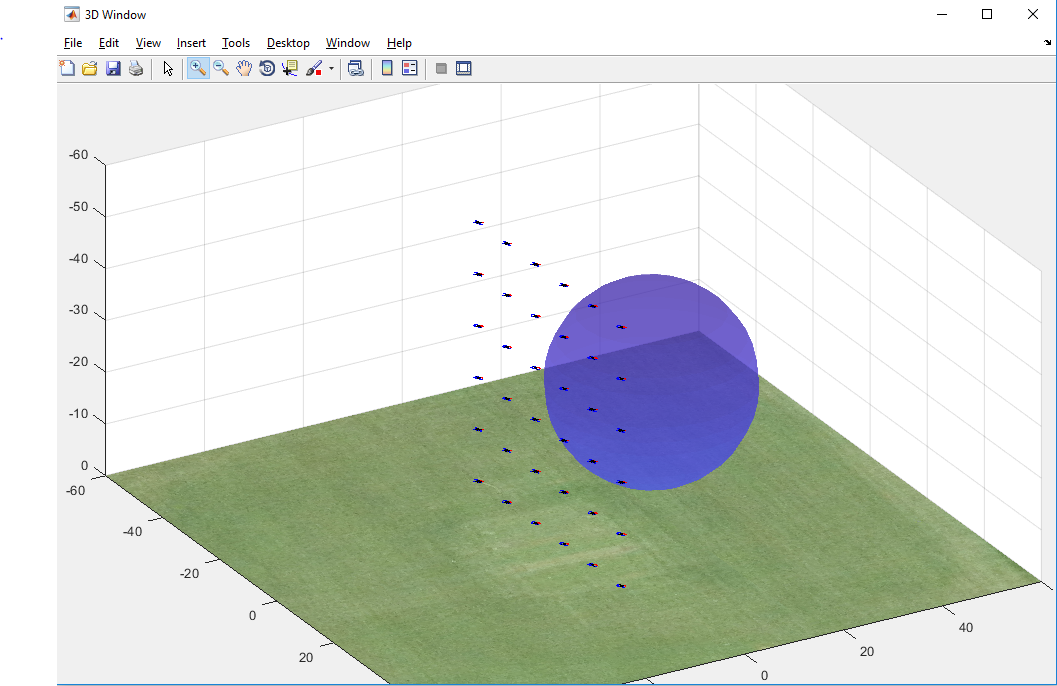
\includegraphics[width=0.8\textwidth]{Chapter-3/figs/initial_drone_config}
\caption{Mesh formation of UAVs at the start of the mission}
\label{fig:mesh_formation}
\end{figure}

\begin{figure}[hbtp]
\centering
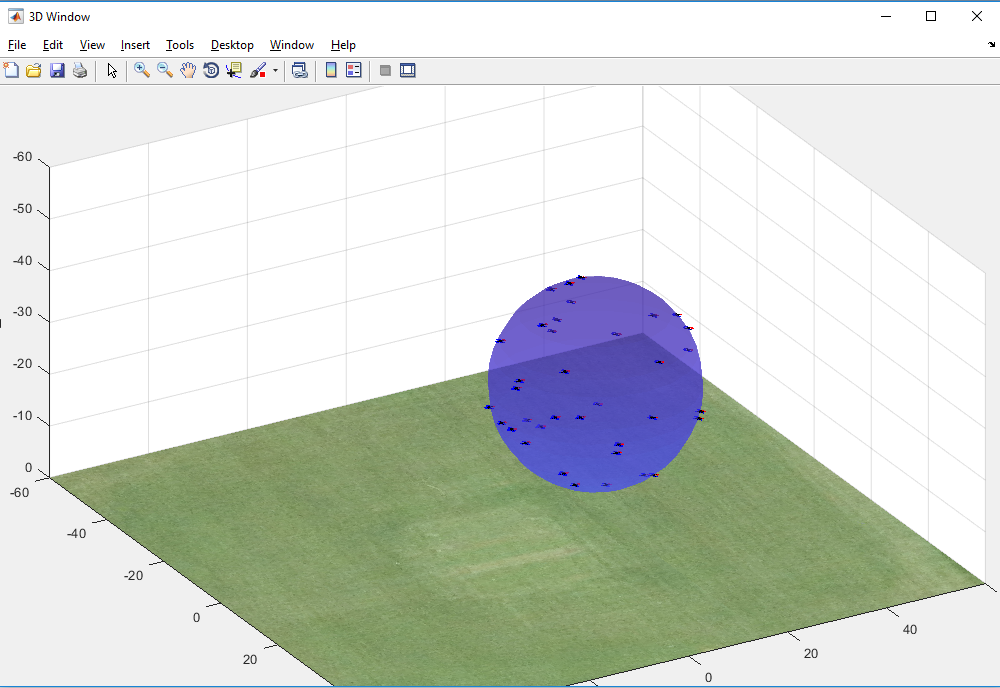
\includegraphics[width=0.8\textwidth]{Chapter-3/figs/final_formation}
\caption{Desired final state of UAVs wrapped around the plume}
\label{fig:final_state}
\end{figure}


\section{Communication requirements} \label{comm_reqs}
\textbf{Content}: There are different network requirements for communicating telemetry/ coordination and sensed data, some of them are delay tolerant and some need to be delivered to a specific region.

\textbf{Intent}: Discuss the scenarios where uav-to-uav, uav-to-ground station unicast would be required and the scenarios where geocast would be suitable. 

In this section, we shall outline the qualitative and quantitative requirements from a communications viewpoint for the successful communication of the mission. We shall use these requirements to design the routing protocol, the message primitives and eventually as a yardstick to measure the performance of the proposed protocol. It should also be noted that the requirements are geared towards a specific mission and since the UAV applications are diverse, these communication demands, and requirements shall widely vary for different applications. For a comprehensive analysis of various civil UAV applications, we refer the readers to \cite{7463007}, where the authors have classified the civil applications of UAVs into four broad categories, namely, Search and Rescue, Area or Network Coverage, Construction, Delivery/transportation and presented the requirements from a communications viewpoint. 

\textbf{Mission coverage:} Applications like plume tracking, wildfire monitoring or plume wrapping typically span a medium to large sized area in the order of tens of kilometers \cite{7463007}. Furthermore, the aerial network should consider the coverage volume expansion or shrinkage with time. The mission volume that we shall be considering would be $ \approx 1500 m \times 1500 m \times 1000 m $. 

\textbf{Network requirement:} Since the mission requires coordination among the participating UAVs, any two participating UAVs should be able to reliably communicate with each other (either directly or multi-hop connectivity). Moreover, the network should be able to reconfigure itself, in other words, the network should consider the nodes joining and leaving the network while the mission is in progress.

\textbf{Number of nodes:} The number of UAVs required in a mission depends on the mission area, transceiver characteristics and the type of nodes employed. Assuming off-the-shelf Wi-fi transceivers and the above mentioned mission coverage the required number of nodes would be around 30. 

\textbf{Connectivity to a base station:} In a real-life deployment scenario, the UAVs must be connected to a base station for safety and security purposes, although the data-rate requirement of the link can be mission specific. In our case, the UAVs need to send their telemetry information (GPS and IMU data) to the base station, however since the mission is fully autonomous with distributed decision-making capacity the entities don’t need to relay the coordination data to the base station. A frequency of 4-5 Hz or less is the standard for telemetry data exchange \cite{7463007}. 

\textbf{Connectivity between the other UAVs:} Since the UAVs are required to maintain an approximate mesh structure they need to approximate the distance with other drones. Therefore, the UAVs need to update each other of their GPS locations in real-time. A suitable frequency of this data exchange could be 4-5 Hz. Also, in real deployment scenarios, the UAV cluster can be composed of drones with varying capabilities (UAVs have different sensors) which demands a need for one-to-one communication. Therefore, the UAVs must have a reliable connectivity to each other in either a single or multi-hop fashion. 

\textbf{Traffic Demands:} The traffic in the aerial UAV network consists of control data (remote controlled data exchange), telemetry data (GPS and IMU data), coordination data (waypoint, mission plan exchange) and sensed data (sensor data). The actual traffic demands depend on the sensor-on-board the UAVs, the type of traffic exchanged in the network and the frequency of such exchange. As per \cite{NASA_UAV_mission_parameters}, imagery and chemical data would need to be collected which would require chemical analyzer, an infrared sensor, image or possibly a video camera. The sensed traffic is sensor dependent and can be, low-rate, bursty or high-rate. In our case, the UAVs need to exchange coordination data among each other, sensed data with the base station and telemetry data with each other as well as the base station. The data exchange with the base station can be periodic and delay-tolerant but the coordination data among the drones must real-time. As far as data rate is concerned 1 Mbps for images and 2 Mbps for video streaming is sufficient with a typical delay of not more thatn 50-100 ms \cite{7463007}. 

\textbf{Collision Avoidance:} Once a UAV detects another UAV (e.g. via RADAR) in its flight path, they both need to navigate around each other to avoid a collision. To check if a future waypoint is void of other UAVs, the source UAV can send an anycast to that specific destination region. If some other UAV happens to be in the region then they should negotiate their way around. It should be noted that the originator UAV doesn't know or care about the identity of the drone, rather the message is addressed to the geographical region. This requires a capability to geocast packets where the destination location is the address. These messages are not delay-tolerant and need to be delivered in real time.

\textbf{Scalability:} The number of nodes can be increased due to two reasons. (1) Increase the coverage volume (2) Increase the density of nodes to get a high-resolution sensory data. A scalabilable network  should handle the increase in a number of nodes/devices in the network and the performance should not degrade unreasonably. 

\textbf{Localization and time synchronization:} The UAVs need to know and report their own location with an accuracy of $\approx 5 m$. This level of accuracy is achievable with off-the-shelf GPS devices and can be improved to a few centimeters by using dual-frequency receivers and/or augmentation systems \cite{gps_accuracy} . The UAVs can also synchronize their clocks through the information provided by GPS.

The above information is summarized in table \ref{tab:communication_requirements}.
\begin{table}
\caption{Communication requirements}
\label{tab:communication_requirements}
\begin{tabular}{|p{0.38\linewidth}|p{0.47\linewidth}|}
\toprule
Requirements & Values\\
\midrule
Mission Coverage & Medium or Large $\approx 1500 m \times 1500 m \times 1200 m$ \\
\midrule
Network mode & ad hoc \\
\midrule
Number of nodes &  $\approx 30 $ \\
\midrule
Coordination data exchange frequency &  4-5 Hz \cite{7463007}\\
\midrule
Sensed data exchange frequency & 30 Hz for video, 1 Hz for IR and chemical analyzer \cite{7463007}\\
\midrule
Telemetry data exchange frequency & 4-5 Hz \cite{7463007}\\
\midrule
Coordination data link rate (up/down) & 4.8 /64 kbaud \cite{7463007} \\
\midrule
Sensed data link rate (up/down) & 4.8-9.6/64 kbaud \cite{NASA_UAV_mission_parameters} \\
\midrule
Delay & 50-100 ms \cite{7463007}\\
\midrule
Traffic type & periodic and real time (coordination data, telemetry data), delay tolerant (sensed data) \\
\bottomrule
\end{tabular}
\end{table}

\section{Routing protocol} \label{routing_protocol}

\textbf{Content: Discuss the location service employed to get destination location, packet header, message primitives and packet routing strategy.}

\textbf{Intent: Explain how a node knows the location of the destination node, and when a node transmits a received message.
}

In this section, we shall first discuss our underlying assumptions in presenting our routing scheme, the packet header and then we shall discuss the message primitives derived from the communication requirements presented in section \ref{comm_reqs}.  

\textbf{Assumptions:}
\begin{enumerate}
\item The wireless antennas on the nodes are omnidirectional.
\item The nodes are reachable from each other i.e. a flooding algorithm can guarantee packet delivery between any pair of nodes and we use the delivery rate of flooding algorithm as an upper bound for our algorithm.
\item The nodes always know their location via GPS. 
\item The nodes synchronize their clock via GPS.
\item A source node knows an approximate location of the destination node which is maintained in a location table and provided by a location service. Different implementations of a location service have been mentioned in section \ref{loc_service} and our implementation has been explained in section \ref{loc_service_impl}. 
\end{enumerate}

\subsection{Packet Header} \label{packet_header}
We first define the packet header that the source node attaches to the payload.
\begin{itemize}
\item Packet ID (\emph{pId}): A number that uniquely identifies this packet among those transmitted by this node. The combination of source node identification and packet ID should uniquely identify a packet in the FANET. 
\item Source Node ID (\emph{srcId}): A unique identifier for the source node. It could be IP address of the node.
\item Source Location (\emph{sLoc}): The GPS coordinate of the source node.
\item Destination Node ID (\emph{destId}): A unique identifier for the destination node. If a packet is destined to a geographical region, then this shall be set to the macro ANY. If a packet is to be flooded in the network, then this value should be set to the macro FLOOD. 
\item Destination Location (\emph{dLoc}): GPS coordinate of the destination as known to the source node. In case of flood packet, this would be set to NULL or be ignored. 
\item Radius (\emph{r}): In case of a geocast packet, the radius along with dLoc defines the destination spherical region for the packet.
\item Transmitter ID (\emph{trId}): A unique identifier for the latest transmitter of the packet.
\item Transmitter Location (\emph{trLoc}): GPS coordinate of the node that had last transmitted the packet.
\item Timestamp (\emph{timestamp}): The time when this packet was transmitted by the source.
\item Width (\emph{w}): The width of the transmission zone for the packet. Explained later in this section.
\item Hops To Live (\emph{HTL}): A node forwards a message only if HTL > 0 and reduces HTL by 1 before forwarding the packet. 
\item Acknowledgement Required (\emph{ackReq}): This flag denotes whether the source node is expecting an \emph{ack} reply.
\item Update Allowed (\emph{update}): This flag denotes whether an intermediate node can update the message headers. For example, if the intermediate node has a location update that is later than the message's \emph{timestamp}.

\end{itemize}

\subsection{Message primitives} \label{message_primitives}

As discussed in section \ref{comm_reqs} the following data exchange happen in the mission:
\begin{enumerate}
    \item UAV to all UAVs: Telemetry data (e.g. GPS, IMU data).
    \item UAV to base station: Telemetry data and sensed data.
    \item UAV to any UAV is a region: Coordination data (e.g. Future waypoint).
\end{enumerate}

To facilitate the above data exchange we should support the following message primitives:
\begin{enumerate}
\item \emph{Flood(message, sourceID)}
\item \emph{Unicast(message, sourceID, destinationID)}
\item \emph{Geocast(message, sourceID, destinationCoordinates, radius)}
\end{enumerate}

Here \emph{sourceID} and \emph{destinationID} are unique identifiers for a node - possibly IP addresses, while \emph{destinationCoordinates} together with \emph{radius} represent a spherical region with specified coordinate as the center and specified radius.

We will now present a high-level algorithmic description of these message primitives.

\paragraph{Flood}

Flood primitive is ensures that the packet shall be received by all the nodes that are connected. When a source node `S' needs to send a message to every node in the network, it creates a header with the following parameters and encapsulates the data in this header.

\begin{eqnarray*}
& header = & messageHeader(destId = FLOOD, dLoc = IGNORE, \\
&    & radius = IGNORE, pdate = IGNORE, width = IGNORE, \\
&    & ackReq = FALSE, HTL = NETWORK\textunderscore DIAMETER)
\end{eqnarray*} 

Node `S' then broadcasts this message to all its neighbors in the wireless medium. An intermediate node 'N', on receiving the message for the first time reads the contents and rebroadcasts it. Thereafter, `N' discards any duplicate receptions of the message. This guarantees that the flooding is loop-free. The benefit of Flooding is the protocol's robustness however there is a high overhead associated with flooding and hence it is suitable for small packets only.

The primitive allows to restrict the span of flooding by the HTL parameter. For example, if a source node `S' wants to send a message to all its immediate neighbors (i.e. in direct radio range) then `S' shall set the HTL value to 1 in the header.

The part of receive algorithm that deals with FLOOD packets is depicted in algorithm \ref{flood_recv}

\begin{algorithm}
\caption{Receive(msg): Flood} 
\label{flood_recv}
\DontPrintSemicolon
\SetKwProg{Receive}{Receive}{}{}
\Receive{(msg)}{%
    \If{msg.pId $\in$ transmittedMsgIdSet}{
        discard(msg)\;
        EXIT\;
    }
    \eIf {msg.destId == FLOOD}{
        \eIf{msg.pId $\notin$ seenIdSet} {
            msg.HTL = msg.HTL - 1\;
            Add (seenIdSet, msg.pId)\;
            \If {msg.HTL > 0}{
                transmit(msg)\;
            }
        }{
            discard(msg)\;
        }
    }{
    ...
    }
}

\end{algorithm}

\paragraph{Geocast}

Geocast is used when a UAV wants to communicate with any node present in a geographic region. This is useful in scenarios where two nodes with a conflicting path and need to communicate to negotiate the path. The underlying mechanism of geocast is flooding but we restrict the flooding to a specific `zone' i.e. if an intermediate node happens to be in that `zone' then only the intermediate node shall re-transmit that message.  

\begin{figure}[hbtp]
\centering
\includegraphics[width=1\textwidth]{Chapter-3/figs/Spheroid}
\caption{Transmission zone with source at sLoc and destination at dLoc}
\label{fig:spheroid}
\end{figure}

\textbf{Transmission Zone:} Consider source node `S' (at \emph{sLoc}) needs to send a message to a destination location \emph{dLoc}. The source node will first create a message (\emph{msg}) and defines a volume in the form of a spheroid with \emph{msg.sLoc} and \emph{msg.dLoc} as the two foci points and parameter \emph{msg.w} as the minor-axis length. An intermediate node `N' forwards this \emph{msg} if and only if `N' lies inside the spheroid defined by the \emph{msg} parameters. This idea of constrained flooding is derived from the concept of the petal in \cite{6133499} and that of request zone in \cite{Ko:1998:LRM:288235.288252}. To increase reliability, the source node can increase the parameter transmission zone's width \emph{msg.w}.

A sample depiction of transmission zone is depicted in \fref{fig:spheroid} where sLoc and dLoc are the foci points and `w' is the length of the minor axis.

When a source node `S' needs to send a message to \emph{any} node in a spherical region `R' with center at \emph{`dLoc'} and radius \emph{`r'} then `S' chooses an appropriate width `w' and creates a header with the following parameters.
\begin{eqnarray*}
& header = & messageHeader(destId = ANY, dLoc = [x,y,z], radius = r,\\
&    & update = IGNORE, width = w, ackReq = FALSE)
\end{eqnarray*}
Source node `S' then encapsulates the data in this header and transmits the packet. An intermediate node `N' processes the message according to the algorithm presented in \ref{geocast_recv}

\begin{algorithm}
\caption{Receive(msg): Geocast} 
\label{geocast_recv}
\DontPrintSemicolon
\SetKwProg{Receive}{Receive}{}{}

\Receive{(msg)}{
    \If{msg.pId $\in$ transmittedMsgIdSet}{
        discard(msg)\;
        EXIT\;
    }
    \If{msg.destId == ANY}{
        \If{insideDestinationRegion(msg, myLoc)}{
            Transmit(msg)\;
            Add msg.pId to transmittedMsgIdSet\;
            EXIT\;
        }
    }
    \If{insideTransmissionZone(msg, myLoc) == TRUE}{
        \eIf{msg.pId is in bufWait}{
            Increase duplicate count for msg.pId\; 
            save msg.tLoc\;
        }{
            boffTime = calculateBoffTime(msg)\;
            add msg to bufWait \;
            
            registerCallback(boffTime, msg)\;
        }
    }
}
\end{algorithm}

\paragraph{Unicast}

Unicast is used when a source node `s' needs to send a message to a destination node `D'. Unicast uses the same underlying mechanism as geocast to route a message except that `S' first consults its location table for `dLoc' - the location of destination `D' - and creates a header with the following parameters.

\begin{eqnarray*}
& header = & messageHeader(destId = destID, dLoc = dLoc,\\
&    & radius = IGNORE, update = IGNORE, width = w, \\
& & ackReq = FALSE)
\end{eqnarray*}

Source node `S' then encapsulates the data in this header and transmits the packet.
An intermediate receiving node `N' follows the algorithm \ref{unicast_recv}.

\begin{algorithm}
\caption{Receive(msg): Unicast} 
\label{unicast_recv}
\DontPrintSemicolon
\SetKwProg{Receive}{Receive}{}{}
\Receive{(msg)}{
    \If{msg.pId $\in$ transmittedMsgIdSet}{
        discard(msg)\;
        EXIT\;
    }
    \eIf{msg.destId = myId}{
        \If{msg.ackReq == TRUE}{
            ackRep = prepareAckReply()\;
            send(ackRep);
        } 
    }
    {
        algorithm \ref{geocast_recv}
    }
}
\end{algorithm}

\chapter{Implementation}

\section{Simulator Introduction: Qrsim} \label{qrsim_intro}
QRSim \cite{denardi2013rn} is a multi-vehicle software simulator developed at Department of Computer Science, University College London. QRSim allows a set of UAVs to communicate and cooperate to achieve common goals. It simulates the dynamics of the UAVs as well as the sensors (GPS, IMU, camera) and the inaccuracies in the sensors and environment (e.g. wind, GPS errors). The simulator also includes the implementation of some specific task scenarios. For example, a pursue evasion game, a search and rescue mission etc. The simulator is specifically helpful in simulating general higher-level tasks that involve multiple platforms which sense and react in their environment. The QRSim has been implemented in MATLAB and the source code is available on GitHub \cite{qrsim_github} under modified BSD license.

We now present a brief overview of the main concepts of the simulator and the relevant classes in its implementation \cite{qrsim_github_manual}.

\paragraph{Platforms and Environment Objects}
\textbf{Platforms} represent quadrotor dynamics and sensor models and other platform specific phenomena like aerodynamic turbulence. Platforms subclass the abstract class Platform (defined in \emph{/qrsim/platforms/Platform.m})

\textbf{Environment objects} represent the phenomena that have a direct or indirect impact of the platforms but are not specific to the platforms like wind or the satellite vehicles of the GPS system or the obstacles in the flight path. Environment objects subclass \emph{EnvironmentObject} (defined in \emph{/qrsim/environment}).
\paragraph{State:} State class maintains the state of all the objects taking part in the simulation. For example, the state structure stores variables like `the simulator time (\emph{t})', `pseudo-random number generator streams (\emph{rStreams})', `the simulator time step (\emph{DT})', `the handle to the 3D graphics visualization (\emph{display3D})'.
\paragraph{Steppable:} Steppable is an abstract class that represents every object that evolves with time. For example, the location of UAV updates after each time quantum (\emph{DT}). Hence the method \emph{step()} exposed by the Steppable class is called which called \emph{update()} on the UAV.
\paragraph{Task:}
Task class allows defining a variety of UAV scenarios and the various objectives for the platforms. The Task class provides a way to derive task objects that specify a scenario and an activity. It exposes methods like \emph{init()}, \emph{updateReward()}, \emph{reward()}, \emph{reset()} and \emph{step()}.
\paragraph{Other abstract classes:}
QRSim API defines several other abstract classes like \emph{AerodynamicTurbulence}, \emph{Sensors}, \emph{AHARS}, \emph{OrientationEstimator}, \emph{Gyroscope}, \emph{Altmeter}, \emph{Accelerometer}.

The main QRSim class defines methods to initialize, set up and control the simulator, namely (a). \emph{init('taskName')} (b) \emph{qrsim.reset()} (c) \emph{qrsim.resetSeed()} (d) \emph{step(U)}.

\section{Qrsim Extensions}

To simulate the message routing protocol and the plume wrapping mission, we had to add/extend some features. In this section, we describe our additions/extensions and our rationale behind our decisions.

\subsection{Radio propagation model} \label{free_space_path_loss}
Our propagation model is based on free space model derived from the Friis transmission formula. \cite{5735774}

The received signal strength $R$ can be calculated as 
\begin{equation}
    R = T - L + N
\end{equation} 
Where,
\begin{itemize}
    \item $R : $ Signal strength at the receiver.
    \item $T : $ Signal strength at the transmitter. (Can be different for each UAV)
    \item $L : $ Path Loss
    \item $N : $ Normal random variable with mean $0$ and standard deviation $\sigma$
\end{itemize}
And Path Loss ($L$) is calculated by the free space path loss equation.
\begin{equation}
 L (dB) = 20 * log_{10} d + 20 * log_{10}(f) + 32.44 - Gt_x - Gr_x 
\end{equation}
Where
\begin{itemize}
    \item $d : $ the distance between the transmitter and receiver (Km)
	\item $f : $ the frequency of transmission (MHz)
    \item $Gt_x : $ the transmitter antenna gain 
    \item $Gr_x : $ the receiver antenna gain.
\end{itemize}

Thereafter, Message Reception Probability $(r) = P(R > R_{th})$. Where $r_{th}$ is the threshold for successful reception of a message. Appropriate values of $T, R, R_{th}$ can be plugged in from the data sheet of WL18xxMOD WiLink\texttrademark Wi-Fi\textregistered   \cite{wilink} (section 5.6 and 5.7 in the data sheet) used in BeagleBone black.

\begin{figure}[hbtp]
\centering
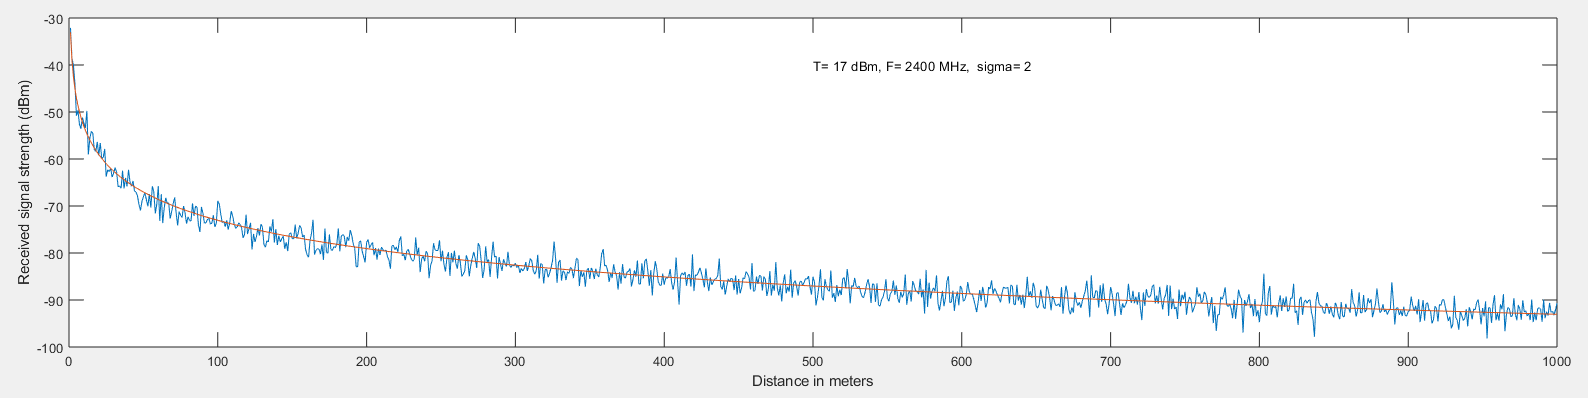
\includegraphics[width=1\textwidth]{ncsuthesis-0.6/Chapter-4/figs/signal_strength}
\caption{Received signal strength vs distance}
\label{fig:signal_strength}
\end{figure}
\begin{figure}[hbtp]
\centering
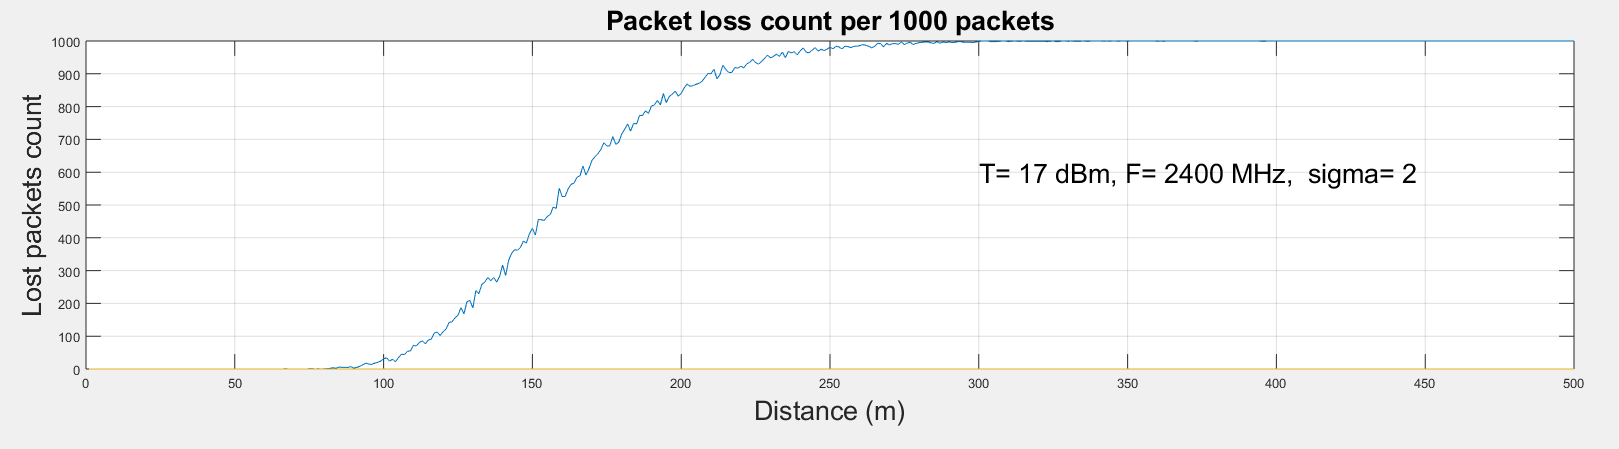
\includegraphics[width=1\textwidth]{ncsuthesis-0.6/Chapter-4/figs/packet_loss}
\caption{Packet loss vs distance}
\label{fig:packet_loss}
\end{figure}
The values used in our simulation are mentioned in \ref{tab:fspl_parameters} and the corresponding received signal strength plot and packet loss plot are shown in \fref{fig:signal_strength} and \fref{fig:packet_loss}:

\begin{table}
\caption{Free space path loss - equation parameters}
\label{tab:fspl_parameters}
\begin{tabular}{|p{0.43\linewidth}|p{0.43\linewidth}|}
\toprule
Parameters & value \cite{wilink}\\
\midrule
Transmitter Strength (T) & 17.1  dBm \\
\midrule
Receiver Threshold ($R_{th}$)	& -87.2 dBm  \\
\midrule
Transmission Frequency (f) & 2400 MHz \\
\midrule
Standard Deviation ($\sigma$) & 2\\
\midrule
Receiver Antenna Gain ($GT_x$) & 0 dBm\\
\midrule
Transmitter Antenna Gain ($GR_x$) & 0 dBm \\
\bottomrule
\end{tabular}
\end{table}


The function to get the signal strength at the destination is algorithm \ref{signalStrength}
\begin{algorithm}
\caption{Signal strength at destination}
\label{signalStrength}
\DontPrintSemicolon
\SetKwInOut{Output}{output}
\SetKwProg{signalStrength}{signalStrength}{}{}

\signalStrength{(T, f, d, $GT_x$, $GR_x$)}{
    \Output{residualStrength: dBm}
    fspl = $ 20 \times \log_{10}(d) + 20 \times log_{10}(f) + 32.44  - GT_x - GR_x$ \;
    
    mean = 0\;
    sigma = 2\;
    N = normrnd(mean, sigma)\;
    residualStrength = T - fspl + N\;
}

\end{algorithm} 


\subsection{Processing delay}

In simulating message transmission we have ignored propagation delay and transmission delay in our calculation. This is because our estimate of packet processing delay at a UAV is much smaller in comparison to the time quantum (DT) in which the QRSim simulator updates the simulation state. DT is a configurable parameter with the default value of 0.2 seconds. Below we present an estimate of the propagation delay, experimental setup and data on the message processing delay (transmission + reception) on a BeagleBone Black device.
\begin{figure}[hbtp]
\centering
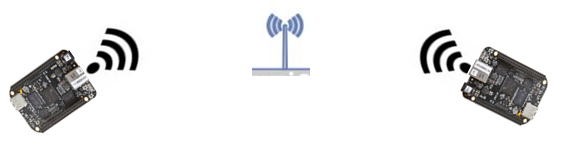
\includegraphics[width=0.8\textwidth]{Chapter-4/figs/beaglebone}
\caption{Measuring processing delay on BeagleBone Black}
\label{fig:proc_delay_setup}
\end{figure}
The setup in \fref{fig:proc_delay_setup} is similar to the configuration proposed in \cite{1378257} to measure network processing delay.

\begin{figure}[hbtp]
\centering
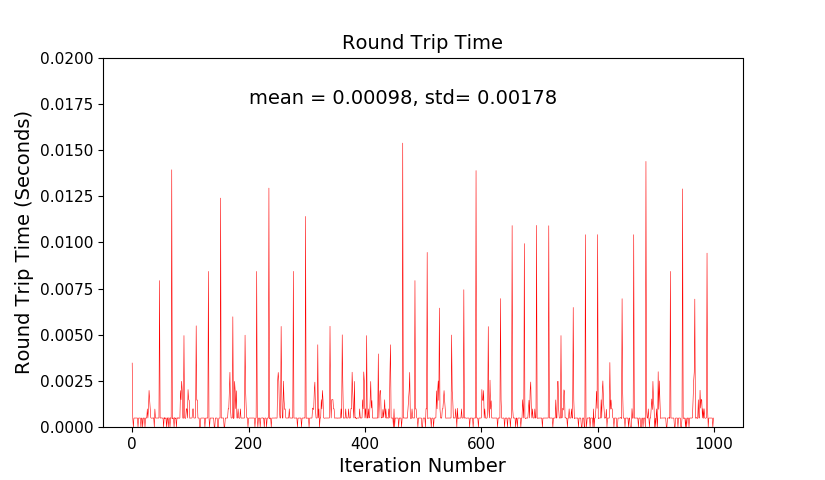
\includegraphics[width=0.8\textwidth]{Chapter-4/figs/transmission_time}
\caption{Round trip time between two BeagleBone Black}
\label{fig:proc_delay_graph}
\end{figure}

A sample plot of round trip time over 1000 iterations is shown in \fref{fig:proc_delay_graph}. It becomes evident that the total message processing delay is much smaller to the time step. Hence, in our simulation, a message transmitted in the time quantum `x' is also received in the same time quantum `x'.

\subsection{Packet Header} \label{packet_header}
We first define the packet header that the source node attaches to the payload.
\begin{itemize}
\item Packet ID (\emph{pId}): A number that uniquely identifies this packet among those transmitted by this node. The combination of source node identification and packet ID should uniquely identify a packet in the FANET. 
\item Source Node ID (\emph{srcId}): A unique identifier for the source node. It could be IP address of the node.
\item Source Location (\emph{sLoc}): The GPS coordinate of the source node.
\item Destination Node ID (\emph{destId}): A unique identifier for the destination node. If a packet is destined to a geographical region, then this shall be set to the macro ANY. If a packet is to be flooded in the network, then this value should be set to the macro FLOOD. 
\item Destination Location (\emph{dLoc}): GPS coordinate of the destination as known to the source node. In case of flood packet, this would be set to NULL or be ignored. 
\item Radius (\emph{r}): In case of a geocast packet, the radius along with dLoc defines the destination spherical region for the packet.
\item Transmitter ID (\emph{trId}): A unique identifier for the latest transmitter of the packet.
\item Transmitter Location (\emph{trLoc}): GPS coordinate of the node that had last transmitted the packet.
\item Timestamp (\emph{timestamp}): The time when this packet was transmitted by the source.
\item Width (\emph{w}): The width of the transmission zone for the packet. Explained later in this section.
\item Hops To Live (\emph{HTL}): A node forwards a message only if HTL > 0 and reduces HTL by 1 before forwarding the packet. 
\item Acknowledgement Required (\emph{ackReq}): This flag denotes whether the source node is expecting an \emph{ack} reply.
\item Update Allowed (\emph{update}): This flag denotes whether an intermediate node can update the message headers. For example, if the intermediate node has a location update that is later than the message's \emph{timestamp}.

\end{itemize}


\subsection{Message transmission}

The Qrsim simulator has a \emph{Pelican} class which represents a quadrotor drone. An object of pelican class stores drone specific data like location coordinates, velocity, rotor thrust etc. To simulate message transmission we added the following properties to the class.
\begin{itemize}
\item transmitter\textunderscore strength
\item receiver\textunderscore threshold
\item transmitter\textunderscore gain
\item receiver\textunderscore gain
\item transmission\textunderscore frequency
\item in\textunderscore msg\textunderscore queue
\item seen\textunderscore msg\textunderscore set
\end{itemize}

When a transmitting node `T' needs to send a message `msg' to a destination `D', the simulation first checks if the signal strength at the destination will be higher than the receiver's threshold (\ref{transmissionSuccess}). If yes, then the simulation appends the message to the in\textunderscore msg\textunderscore queue of the destination node. (\ref{sendMessage})

\begin{algorithm}
\SetAlgoLined
\DontPrintSemicolon
\KwResult{transmissionSuccess: TRUE/FALSE}
transmissionSuccess = FALSE\;
d = distance(T.location, D.location)\;
f = T.transmission\textunderscore frequency\;
ts = T.transmitter\textunderscore strength\;
gTx = T.transmitter\textunderscore gain\;
gRx = D.receiver\textunderscore gain\;
receiverThreshold = D.receiver\textunderscore threshold\;
strength = signalStrength(ts, f, d, gTx, gRx)\;
\If {strength > receiverThreshold}{
    transmissionSuccess = TRUE\;
}

\caption{transmissionSuccess(T, D)} \label{transmissionSuccess}
\end{algorithm}

\begin{algorithm}
\KwResult{status: TRUE/FALSE}
\DontPrintSemicolon
status = FALSE\;
\If{msg.HTL <= 0}{EXIT\;}
msg.HTL = msg.HTL - 1\;
\If{transmissionSuccess(T, D) == TRUE}{
append(D.in\textunderscore msg\textunderscore queue, msg)\;
status = TRUE\;
}

\caption{sendMessage(msg, T, D)} \label{sendMessage}
\end{algorithm}


A receiver iterates over each message in its message queue and discards any duplicate messages. For new messages, the node does the required processing according to the message header and adds the \emph{msg.pId} to the \emph{seen\textunderscore msg\textunderscore set}. Algorithm readMessages \ref{readAllMessages}

\begin{algorithm}
    \caption{Read and process the messages in a drone's buffer} 
    \label{readAllMessages}
    \DontPrintSemicolon
    \SetKwInOut{Input}{inputs}
    \SetKwProg{readMessages}{readMessages}{}{}
    
    \readMessages{(drone)}{
    \Input{drone object of class Pelican}
    \ForEach {msg $\in$ drone.in\textunderscore msg\textunderscore queue}{%
        \eIf{msg $\in$ drone.seen\textunderscore msg\textunderscore set}{%
            discard(msg)\;
        }{
            processMessage(msg)\;
            add(drone.seen\textunderscore msg\textunderscore set, msg)\;
            }
        }
    }
\end{algorithm}

\subsection{Inter-UAV forces}
The UAVs are initially arranged in a grid and then this grid is maintained during the mission. To maintain the grid formation whenever two UAVs, go out of a certain range, they exert a virtual pull towards each other, and when they come too close they exert a virtual push towards each other. Moreover, once two UAVs are beyond a certain limit, their influence should gradually wear off. We use the following sigmoid function to calculate the push or pull force. 
\begin{equation}
    Y = \frac{X}{1 + |X|}
\end{equation}

\fref{fig:force_fn} shows a plot of the force magnitude as a function of distance.

\begin{figure}
\centering
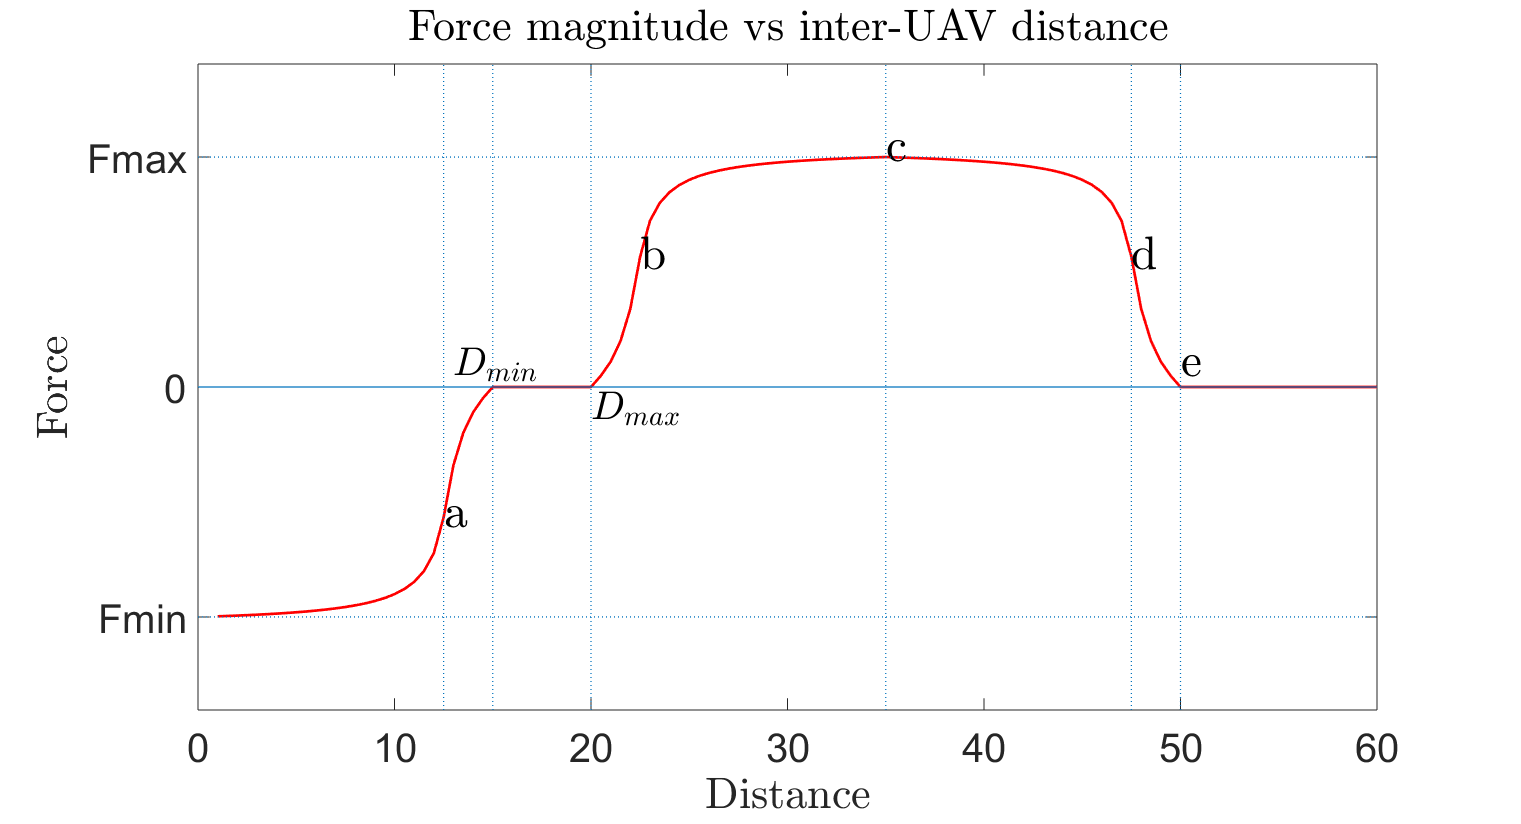
\includegraphics[width=1\textwidth]{ncsuthesis-0.6/Chapter-4/figs/force_function}
\caption{Inter UAV force vs distance}
\label{fig:force_fn}
\end{figure}


\subsection{Location service} \label{loc_service_impl}

For the geographical routing protocols to work successfully, the source node needs to know the geo-location (or an approximation) of the destination location. To provide this information we need a service that maintains and distributes the location table. Some of the proposed location service algorithms have been mentioned in section \ref{loc_service}. In our simulation we have implemented an all-for-all location service i.e. every node maintains the location information of every other node in the network. 

We have employed a hop limited broadcast algorithm to distribute the location table, i.e. in each time step, every node broadcasts its location table to the nodes in its transmission range. The receiving node `R' checks if the location of a node `N' in the message and the timestamp of when the information was generated. If the location in the message is new, then `R' updates its location table. It should be noted that the nodes don't transmit the message again. This is achieved by setting the `HTL' parameter in the message header to 1. It should be noted that a fast moving node can choose to increase the HTL to cover a larger volume in the same time-step.

The effect is that two nodes `p' and `q' which are `x' transmission ranges apart will have a location information that is $x \cdot DT $ time steps old and therefore not an exact but rather an approximate location of each other. The motivation for this implementation is derived from the concept termed as `distance effect' in \cite{Basagni:1998:DRE:288235.288254}, which states
\begin{quotation}
The greater the distance separating two nodes, the slower they appear to be moving with respect to each other. Thus, nodes that are far apart, need to update each other's location less frequently than nodes closer together.
\end{quotation}
However, in \cite{Basagni:1998:DRE:288235.288254} the authors have associated an `age' with the messages which determines how far a message should be transmitted from the source location and the nodes periodically send messages with `large' and `small' age. However, in our case, the information flows gradually like waves in each time-step.

\subsection{Transmission Zone}

As detailed in section \ref{routing_protocol} the idea behind our routing algorithm is to restrict retransmissions to only those nodes that are inside a region. Among the choices presented in section \ref{protocol_description} we have chosen a spheroid volume as our transmission zone because such a volume is a generalization of the other three, provides a tapered region and gives equal significance to nodes at the same distance from the `source - destination' line. As depicted in fig \fref{fig:spheroid} the spheroid has sLoc(p, q, r) and dLoc(a, b, c) as their foci points and `pkt.w' as its minor axis length. An intermediate node `N(x, y, z)' shall forward a message if and only if N is inside the spheroid. We check for this condition using the definition of the ellipsoid `The sum of the distances to the two foci points is constant for every point on the curve.'
\begin{equation} \label{ellipsoid_equation}
    distance(N, sLoc) + distance(N, dLoc) == K
\end{equation}

where $K$ is the length of the major-axis. Hence, if the left hand side of equation \ref{ellipsoid_equation} is $\leq K$ then, the point N is inside the spheroid.

\paragraph{Diffused transmission zone:}
\label{diffuse_trans_zone}
We observe that there are at least two scenarios where the above described transmission zone might not contain the intermediate nodes for successful transmission. 
\begin{enumerate}
    \item Outdated destination location: As discussed in section \ref{loc_service_impl}, if two UAVs are are multi-hops away then they might not have an exact location of each other rather an approximate location which is a few time-steps old. In those cases the intermediate UAVs might have an updated location information. 
    
    \item Routing void: is encountered when there are insufficient nodes close to the `source - destination' line for a successful packet delivery however there are nodes outside the periphery of the transmission zone which can deliver the packets.  
\end{enumerate}

\begin{figure}[hbtp]
\centering
\includegraphics[width=1\textwidth]{Chapter-4/figs/Spheroid}
\caption{Transmission zone with source at sLoc and destination at dLoc}
\label{fig:spheroid}
\end{figure}

\begin{figure}[hbtp]
    \centering
    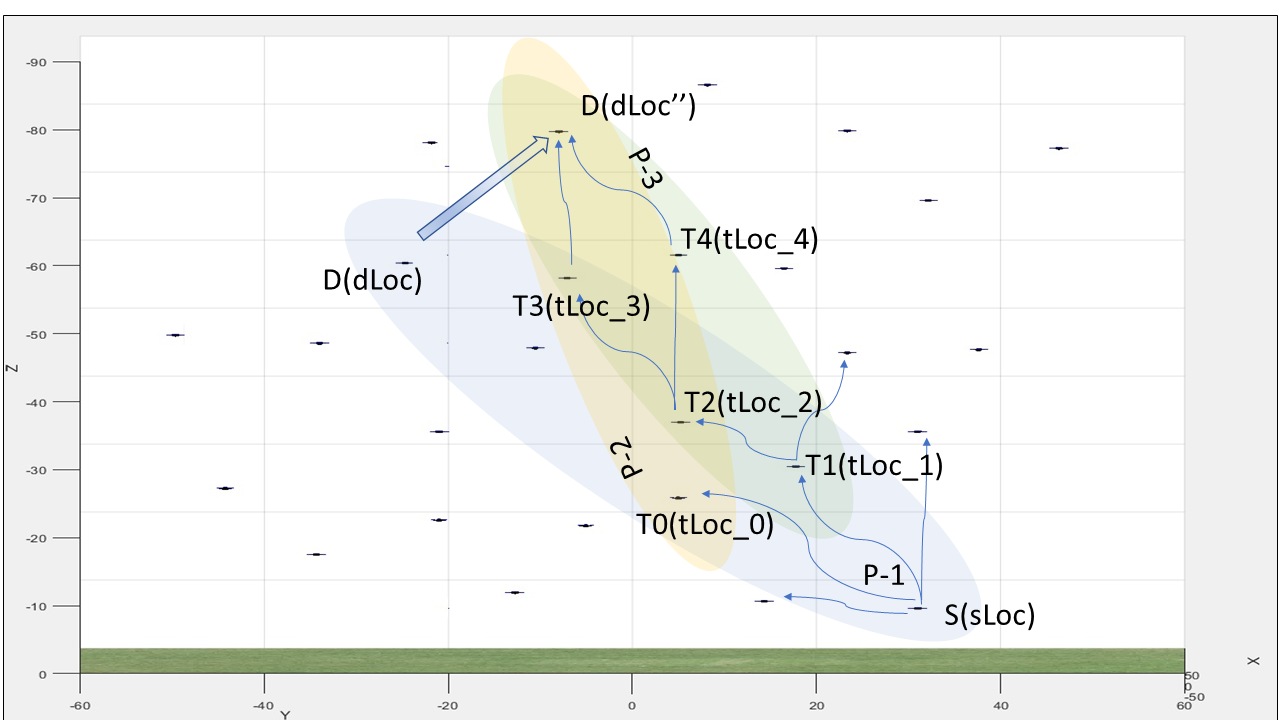
\includegraphics[width=1\textwidth]{Chapter-4/figs/diverge_zone}
    \caption{Diverged transmission zone}
    \label{fig:diverged_transmission_zone}
\end{figure}

In these two cases the source node can increase the zone width which has a disadvantage of increasing the number of transmissions. Another approach is to let the intermediate nodes update the packet headers with newer information. For example, in \fref{fig:diverged_transmission_zone}, the source node `S' needs to send a packet to destination node `D'. `S' creates a packet with headers that specify the zone `P-1' around `sLoc - dLoc'. The intermediate nodes `T0' and `T1' know the current location of D and update the packet with headers that specify zones `P-2' and  `P-3'. Afterward `T3' and `T4' receive the packet and being inside the updated zones transmit the packet which is received by the destination D at `dLoc'''. These approach makes the zones to diverge from the original one and hence we will refer to this scheme as \textbf{diverge zone routing}. This approach also helps navigate the routing void with a thinner zone width as compared to the single zone scheme. 

\textbf{Transmission Zone:} Consider source node `S' (at \emph{sLoc}) needs to send a message to a destination location \emph{dLoc}. The source node will first create a message (\emph{msg}) and define a volume in the form of a spheroid with \emph{msg.sLoc} and \emph{msg.dLoc} as the two foci points and parameter \emph{msg.w} as the minor-axis length. An intermediate node `N' forwards this \emph{msg} if and only if `N' lies inside the spheroid defined by the \emph{msg} parameters.

\subsection{Back-off time}
\label{back_off_time}

We discussed in section \ref{protocol_description}, that the number of transmissions can be further decreased by making the node \emph{back-off} for a certain time and then decide whether to transmit or not. In this section we shall describe the method of calculating the back-off duration. 


\begin{figure}[hbtp]
    \centering
    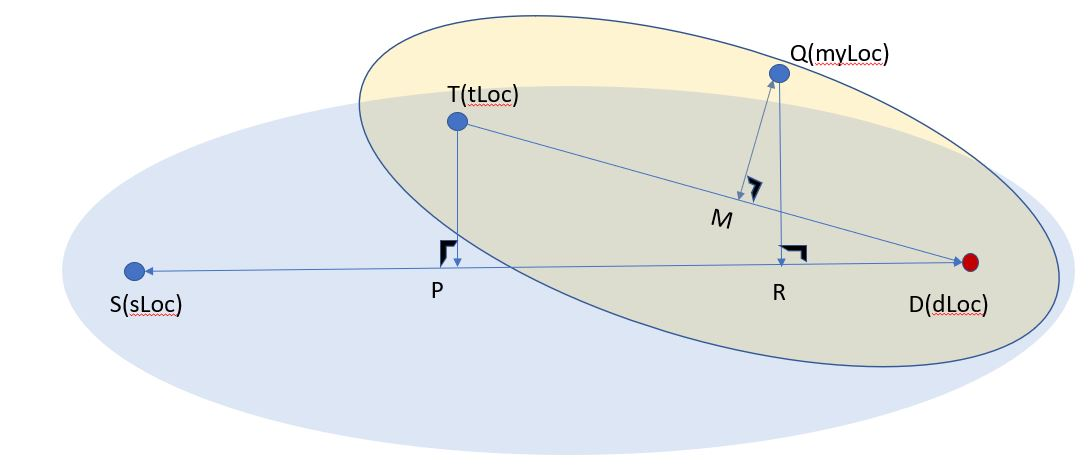
\includegraphics[width=1\textwidth]{Chapter-4/figs/back_off_time_calc}
    \caption{Back-off time calculation}
    \label{fig:back_off_time_calculation}
\end{figure}


The main goal of back-off calculation is that the node closer to the destination and the source - destination line should transmit first. Therefore, the \emph{backOff} calculation is divided into two parts.
\begin{itemize}
    \item tB1 $\rightarrow$ back-off time proportional to the distance from destination. This is bounded above by $tUb1$. 
    \item tB2 $\rightarrow$ back-off time proportional to the distance from the source - destination line. This is bounded above by $tUb2$.
\end{itemize}

For example, as depicted in \fref{fig:back_off_time_calculation}, intermediate node T needs to determine the back-off time. Node T uses the displacement across the SD line (i.e. PD) to calculate `tB1' and then uses the distance from SD line (i.e. TP) to calculate `tB2'.
In case of diverge transmission zone the intermediate node uses the distance from `transmitter - destination' line to calculate `tB2'. This is depicted in algorithm \ref{back_off_time_algo}.

\begin{algorithm}
\caption{Back-off time calculation at intermediate nodes}
\label{back_off_time_algo}
\DontPrintSemicolon
\SetKwInOut{Output}{output}
\SetKwProg{BackOff}{BackOff}{}{}

\BackOff{(sLoc, dLoc, tLoc, myLoc, tUb, tUb1, zoneType)}{
    \Output{backOff seconds}
    
    TD' = projection of $\overrightarrow{TD}$ on $\overrightarrow{SD}$\;
    
    tB1 = $\dfrac{tUb * TD'}{SD}$\;
    
    \eIf {zoneType = SINGLE}{
        X = sLoc \;
        }{
        X=tLoc \;
    }
    
    XP = distance of X from $\overrightarrow{XD}$\;
    
    tB2 = $\dfrac{tUb1 * XP}{XD}$\;
    
    backOff = tB1 + tB2 \;
    }

\end{algorithm} 

\chapter{Performance Evaluation}
\section{Delivery Ratio}
\section{Average number of Hops}
\section{Average End to End Delay}
\section{Overhead}

\chapter{Conclusions and Future Work}


%\restoregeometry


%%---------------------------------------------------------------------------%%
%%  Bibliography 

%% or use BibTeX
%\bibliography{Ortiz-thesis}{}
%\bibliographystyle{plain}
%\nociterec{*}

%\bibliographystyle{plainnat}%plainnat is necessary to enable the use of citet. Natbib style file.
%\bibliography{Ortiz-thesis2}
%\ensureoddstart
\begin{spacing}{1}
 \setlength\bibitemsep{11pt} %22pt = 2*11pt, where fontsize is 11pt
 \addcontentsline{toc}{chapter}{{\uppercase{\bibname}}} %\textorpdfstring and \uppercase needed due to hyperref package http://www.latex-community.org/forum/viewtopic.php?f=44&t=16601
 %\vspace{-0.5in}
\titleformat{\chapter}[display]{\bf\filcenter
}{\chaptertitlename\ \thechapter}{11pt}{\bf\filcenter}
\titlespacing*{\chapter}{0pt}{-0.5in-9pt}{22pt}

\printbibliography[heading=myheading]
\end{spacing}
%\bibliographystyle{apalike}



%%---------------------------------------------------------------------------%%
% Appendices
%\ensureoddstart
\restoregeometry
\appendix
\newgeometry{margin=1in,lmargin=1.25in,footskip=\chapterfootskip, includehead, includefoot}


\chapter{Sample Performance Metrics}

In this section, we present the results of 1 pair of nodes which are furthest apart in the simulation for the three formations. There are 36 nodes in the simulation.

\newgeometry{margin=1in,lmargin=1.25in,footskip=\chapterfootskip, includehead, includefoot}
%\thispagestyle{lscaped}
%\pagestyle{lscaped}
\thispagestyle{lscapedplain}

\begin{landscape}
\begin{figure}
\centering
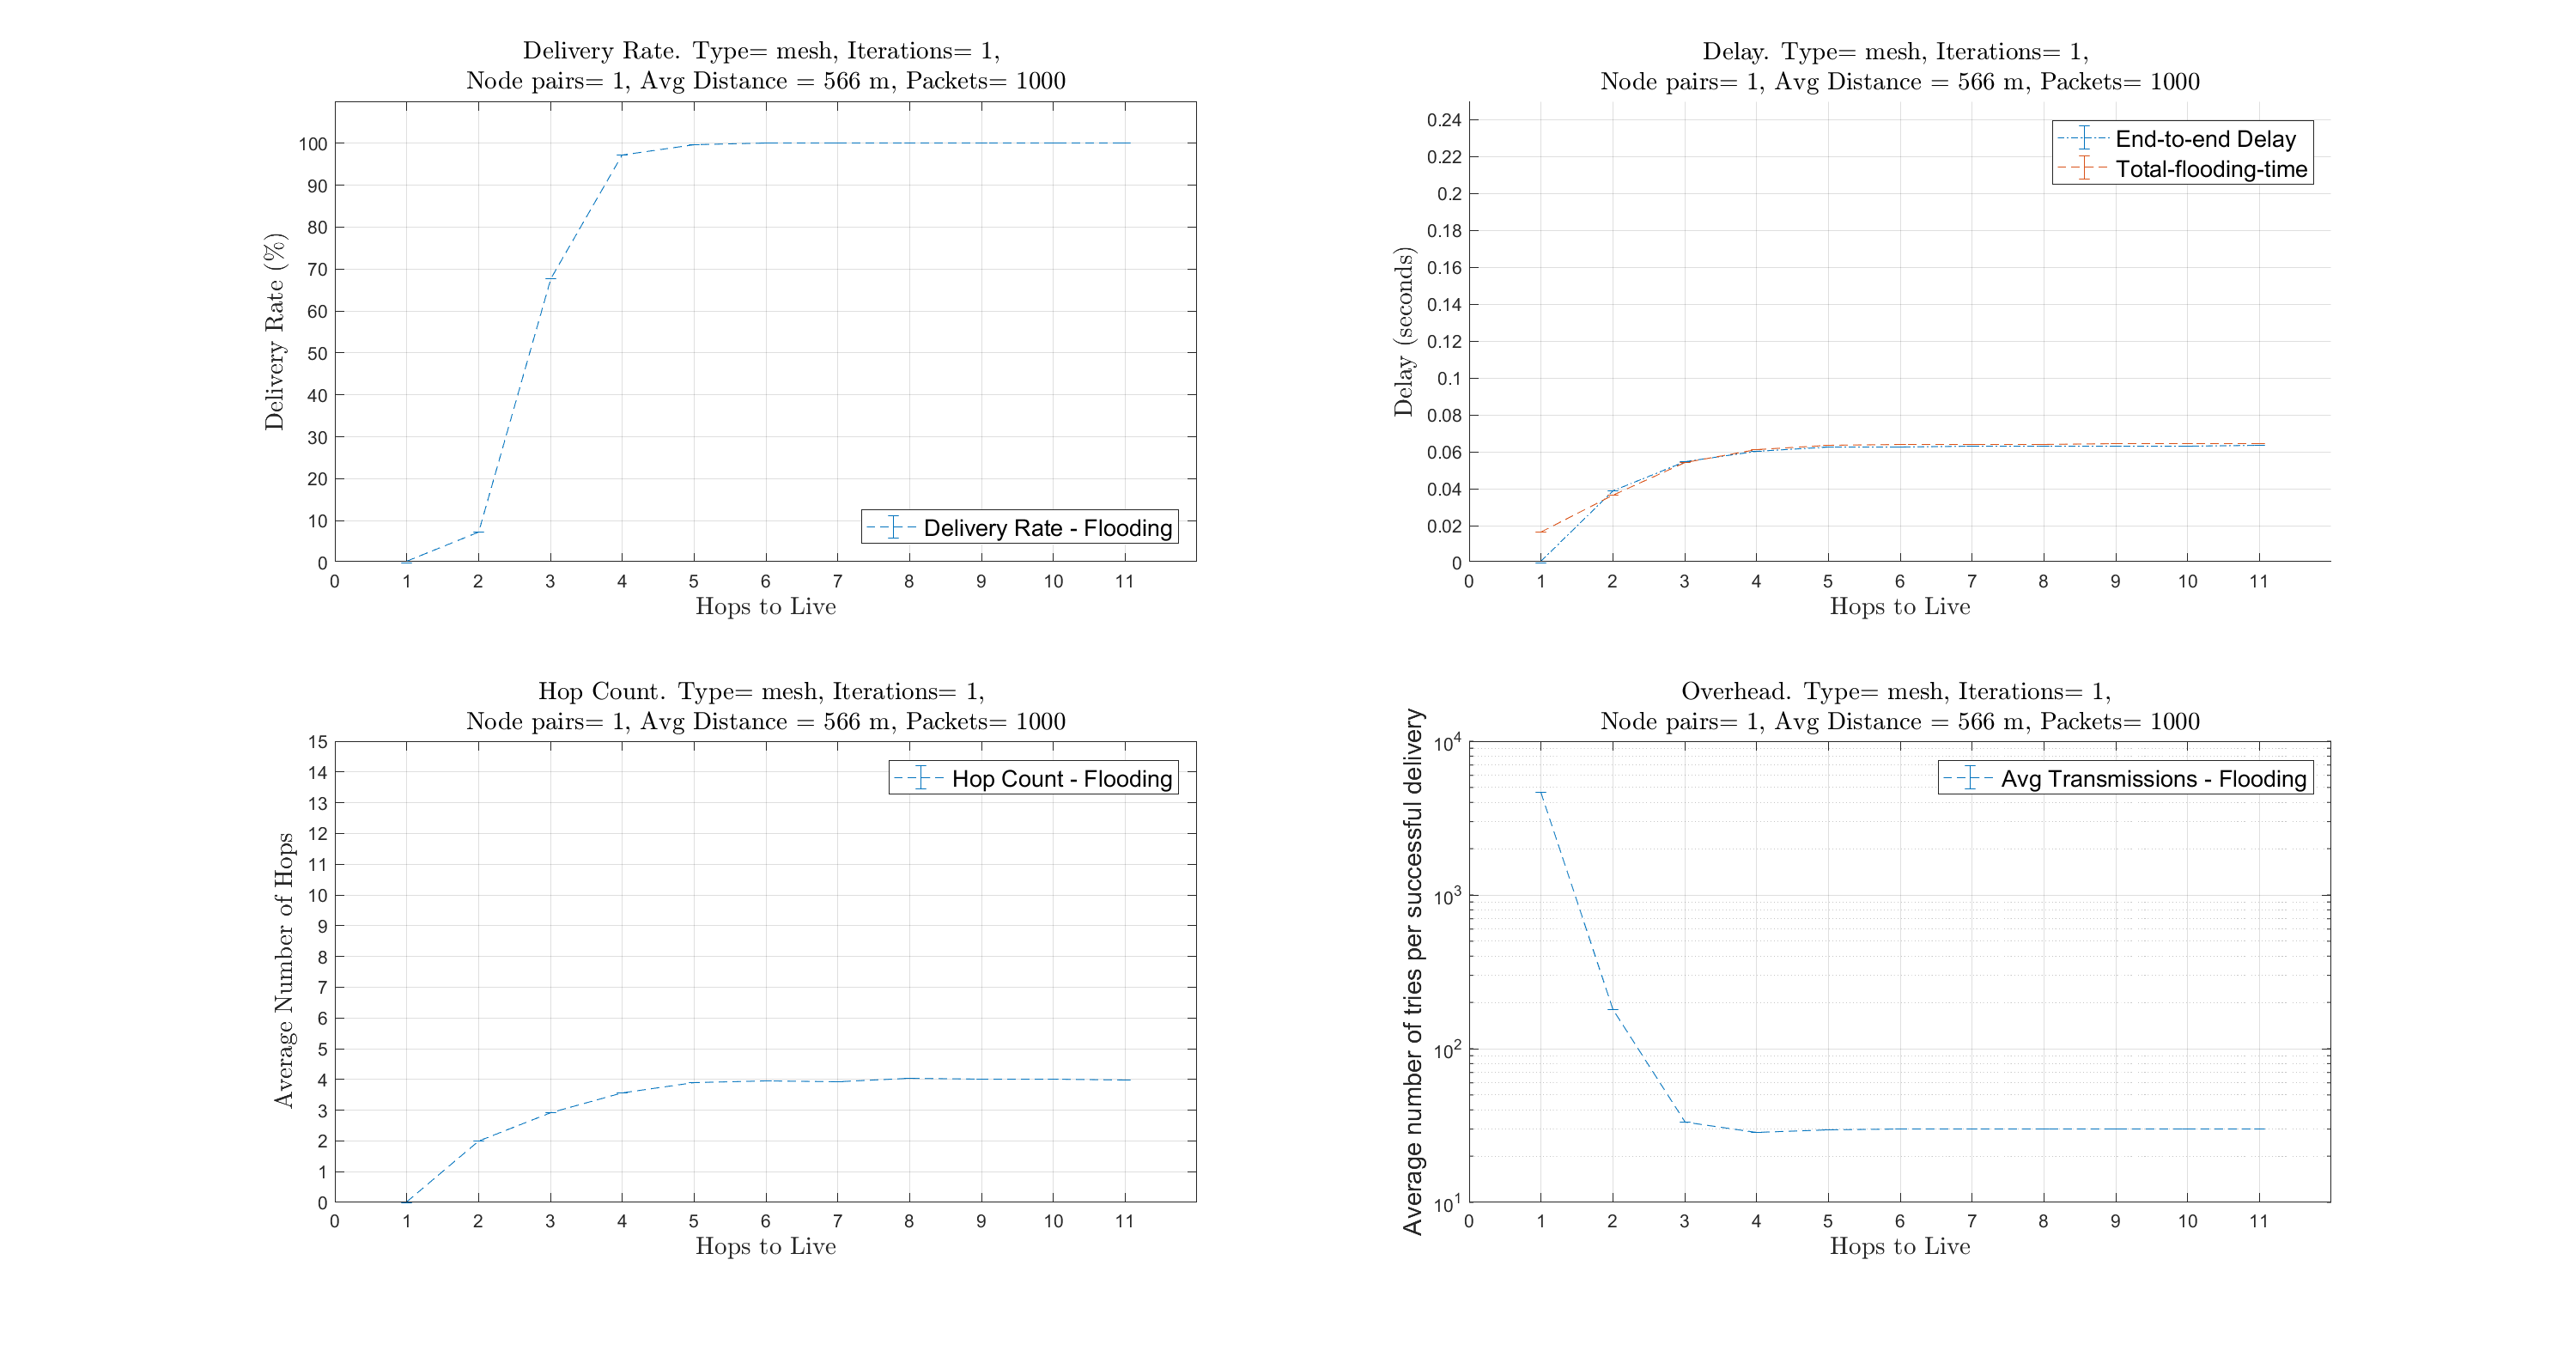
\includegraphics[width=1\textwidth]{ncsuthesis-0.6/Appendix-A/figs/flood_mesh}
\caption{Delivery ratio, end-to-end delay, hops and overhead for flooding algorithm in a 2 dimensional formation of UAVs.}
\label{fig:flood_mesh}
\end{figure}
\end{landscape}

\thispagestyle{lscapedplain}
\begin{landscape}
\begin{figure}
\centering
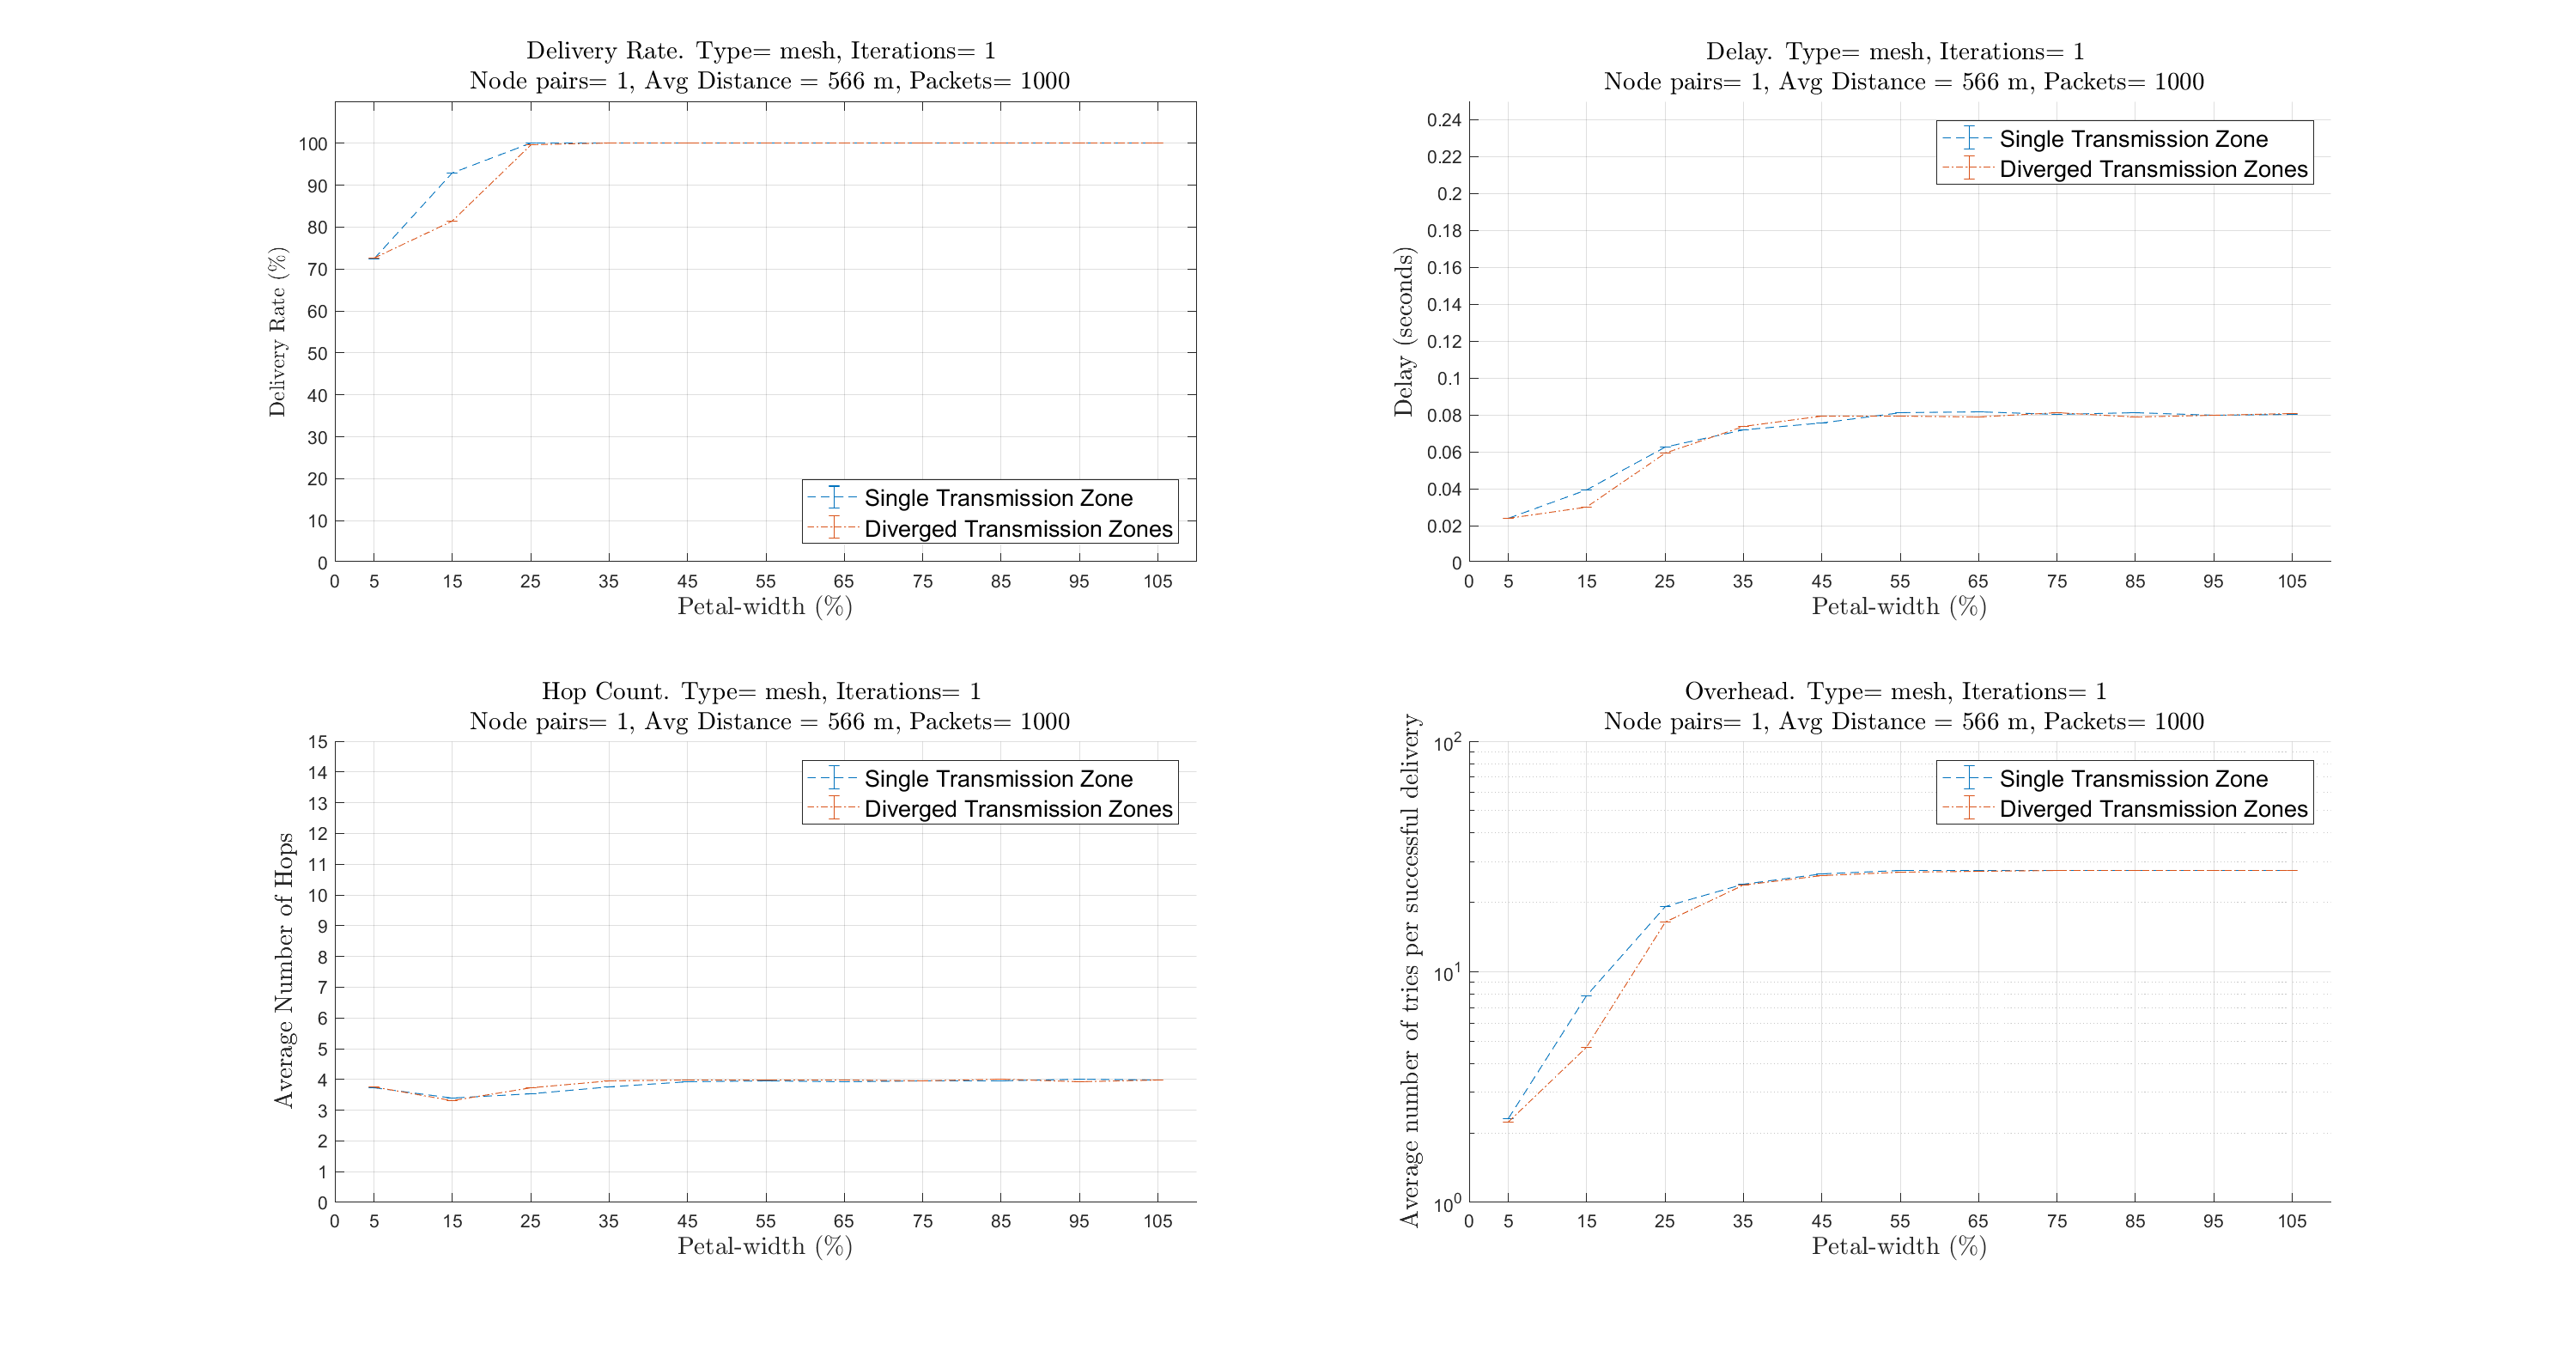
\includegraphics[width=1\textwidth]{ncsuthesis-0.6/Appendix-A/figs/petal_mesh.png}
\caption{Delivery ratio, end-to-end delay, hops and overhead for petal routing in a 2 dimensional formation of UAVs.}
\label{fig:petal_mesh}
\end{figure}
\end{landscape}

\thispagestyle{lscapedplain}
\begin{landscape}
\begin{figure}
\centering
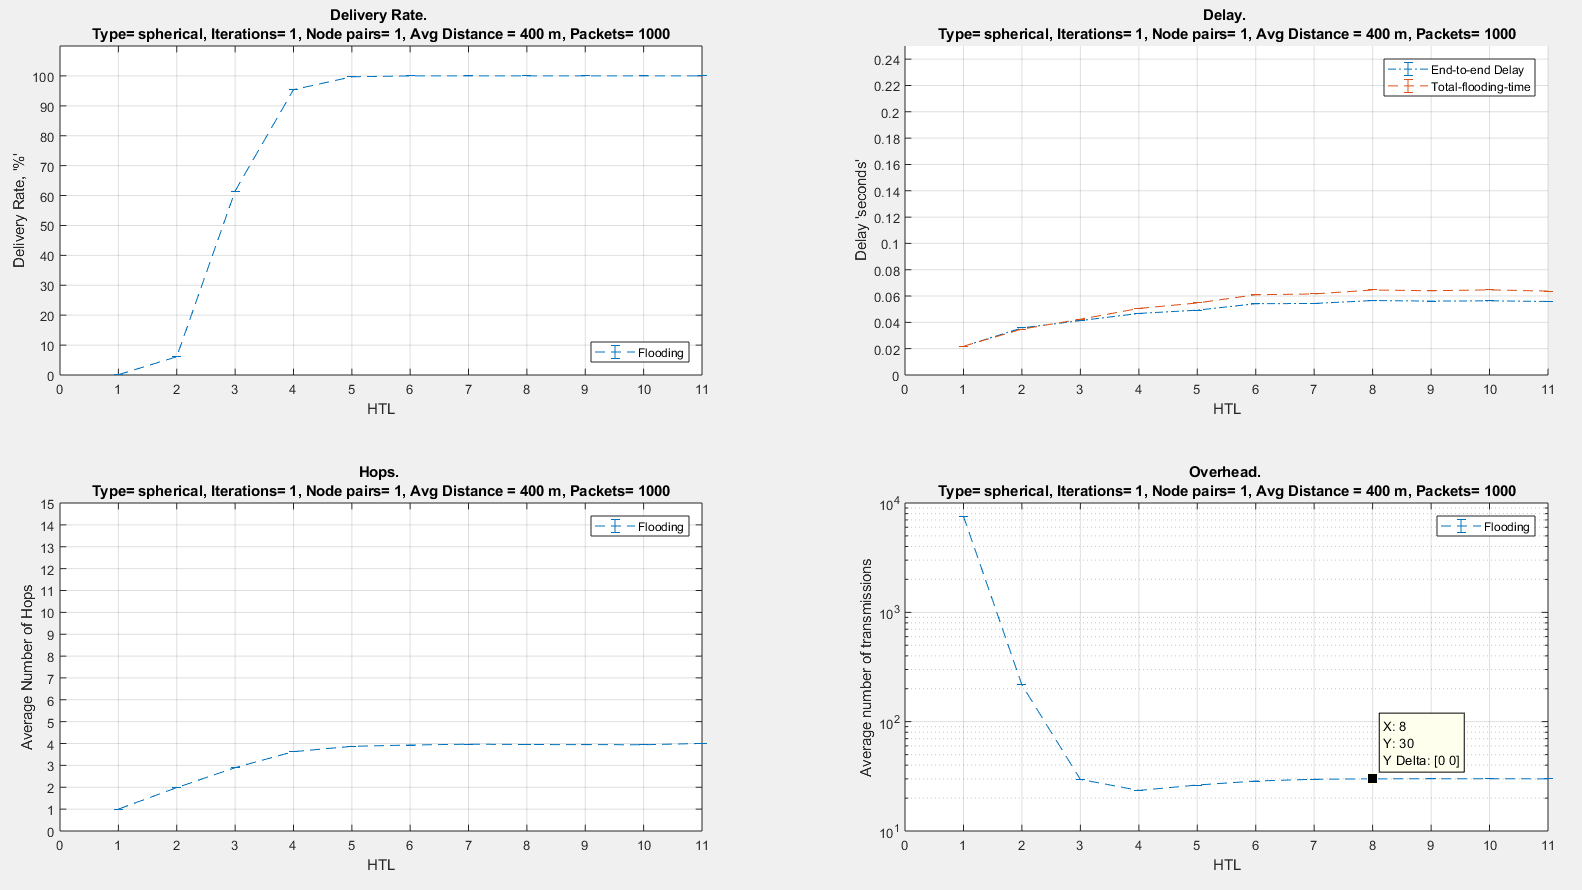
\includegraphics[width=1\textwidth]{ncsuthesis-0.6/Appendix-A/figs/flood_spherical.png}
%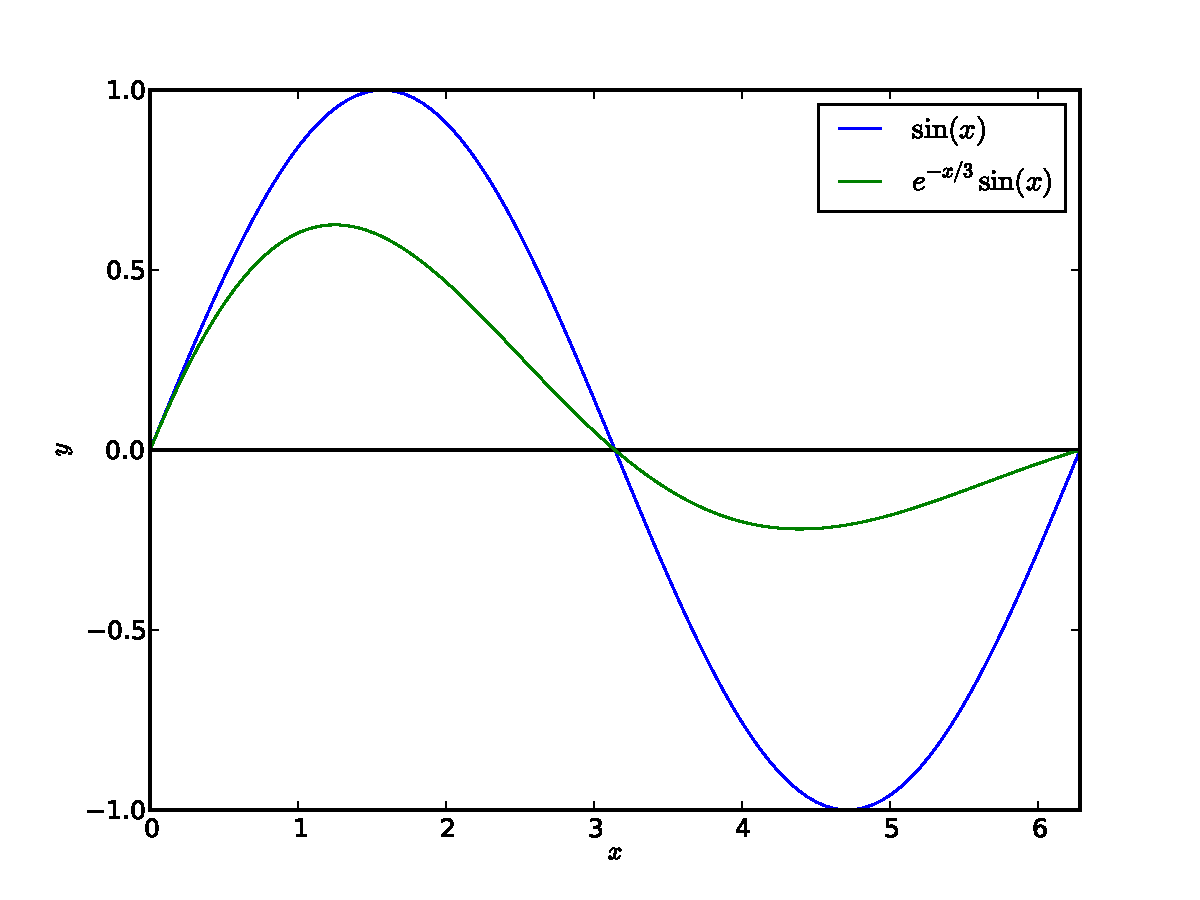
\includegraphics[height=\textwidth]{Chapter-2/figs/sine}
\caption{Delivery ratio, end-to-end delay, hops and overhead for flooding algorithm in a spherical arrangement of UAVs. }
\label{fig:flood_spherical}
\end{figure}
\end{landscape}

\thispagestyle{lscapedplain}
\begin{landscape}
\begin{figure}
\centering
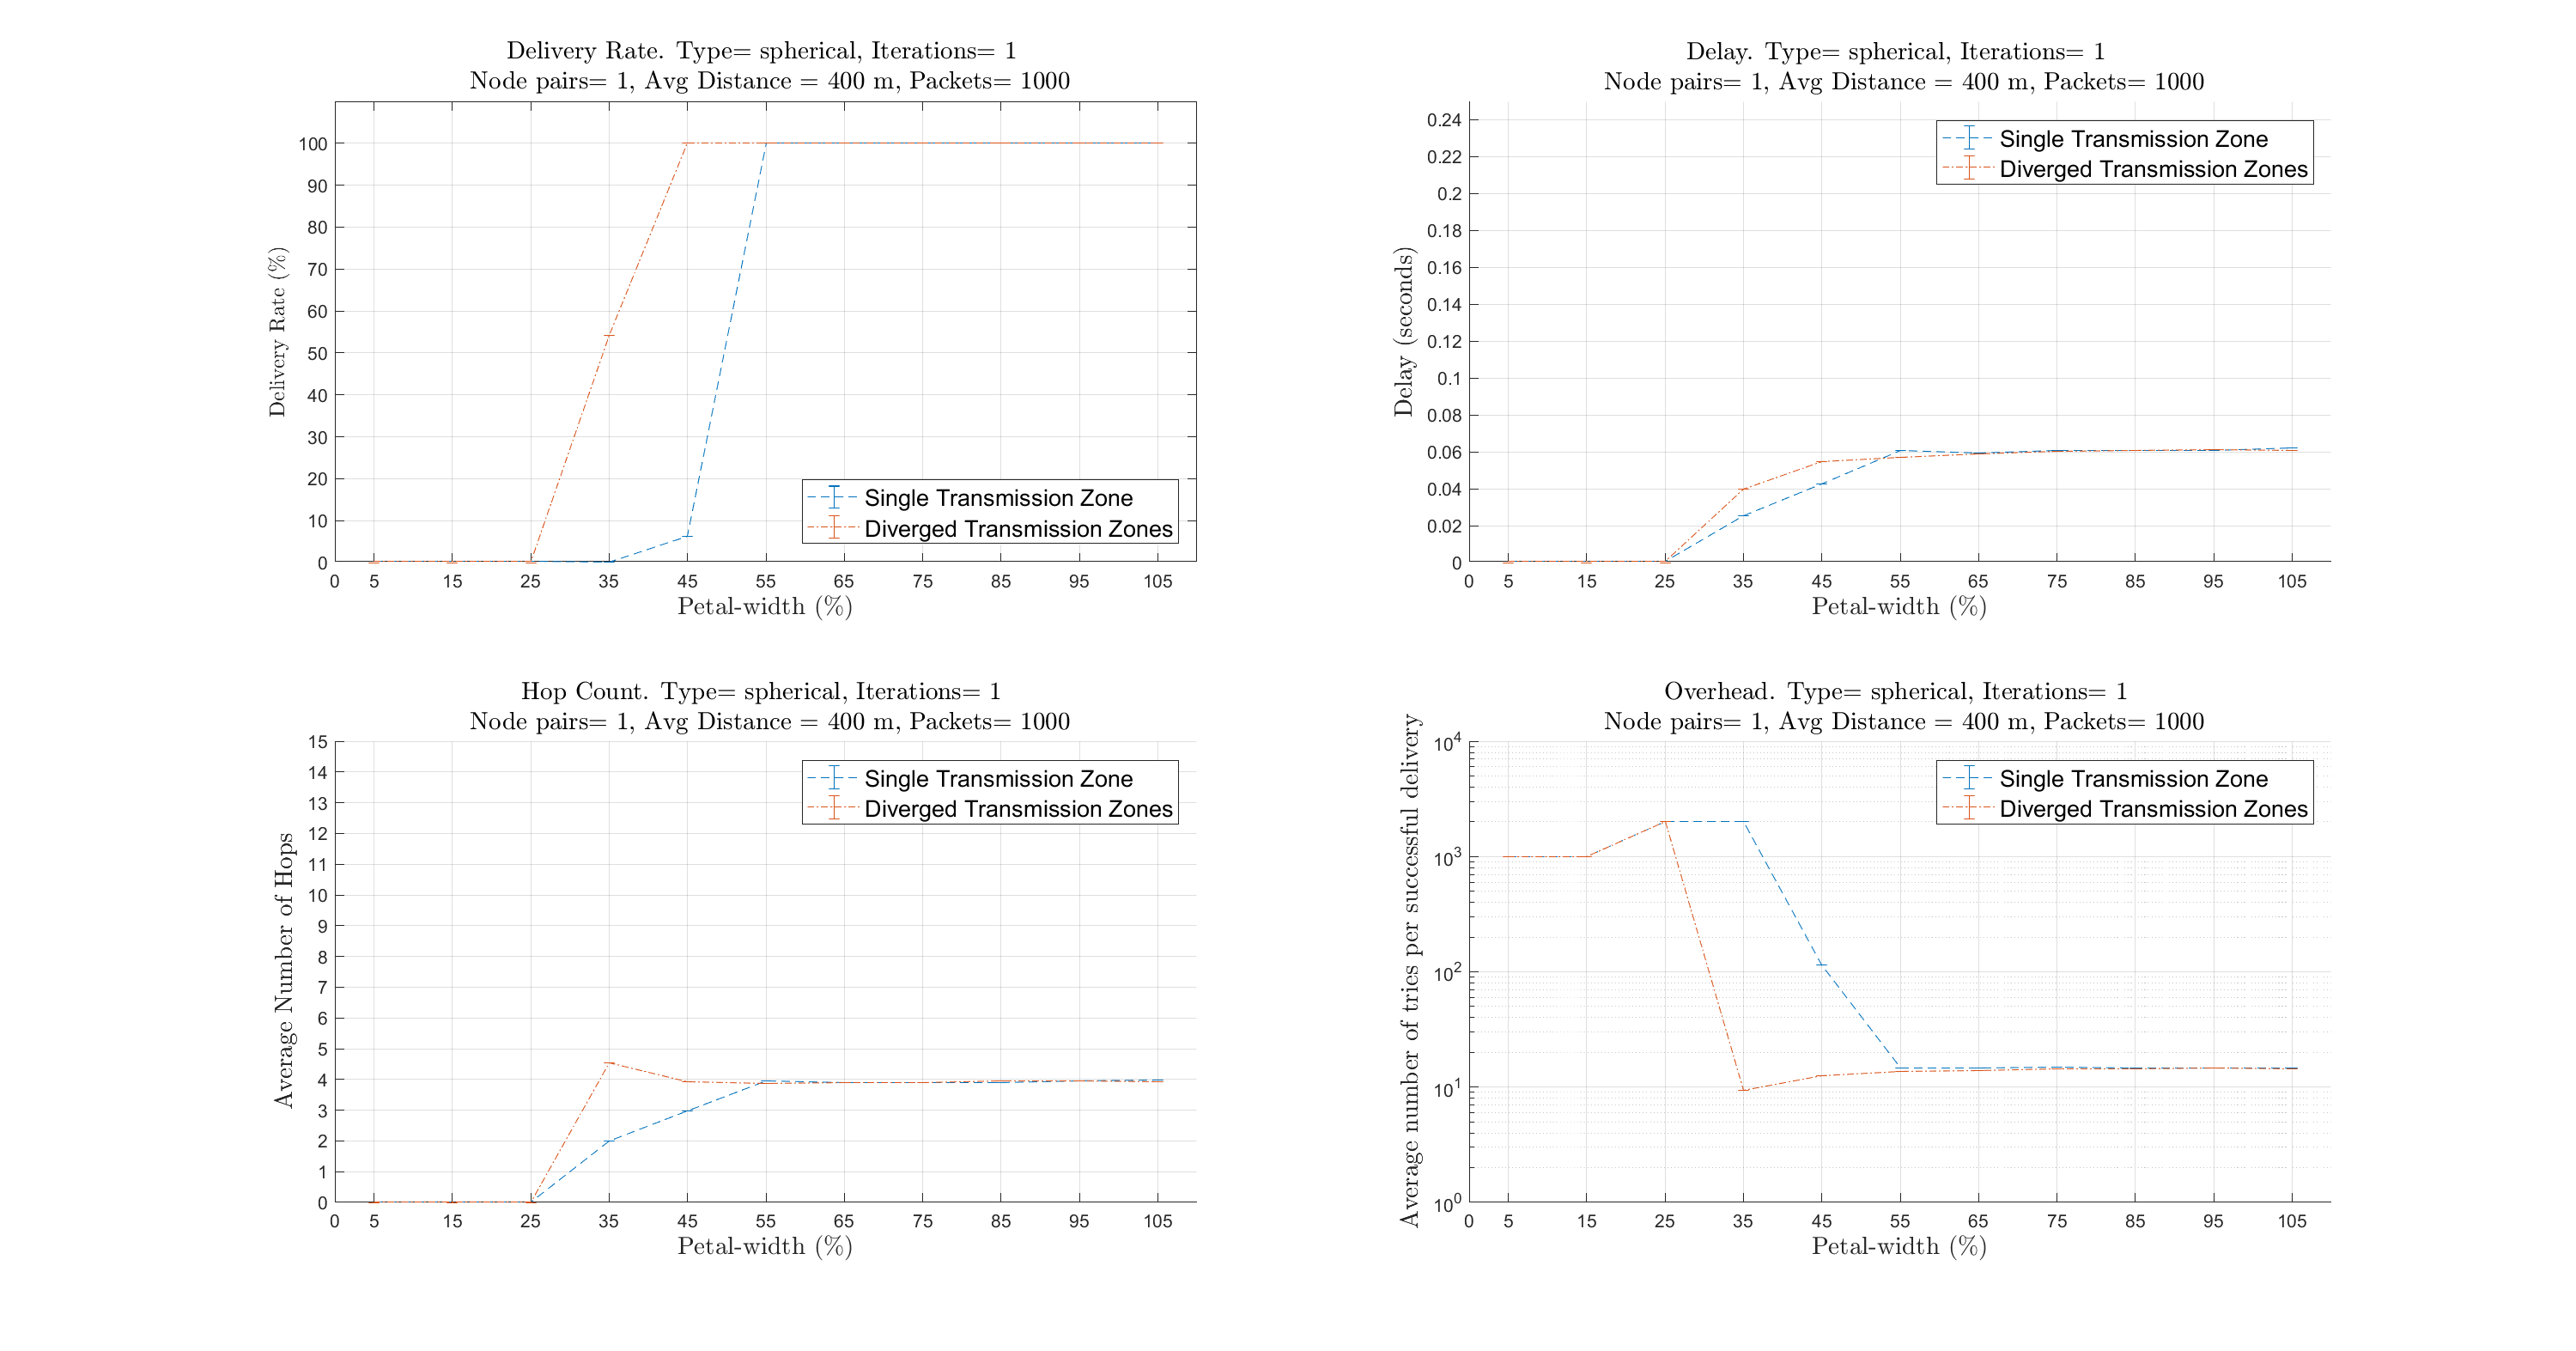
\includegraphics[width=1\textwidth]{ncsuthesis-0.6/Appendix-A/figs/petal_spherical.png}
%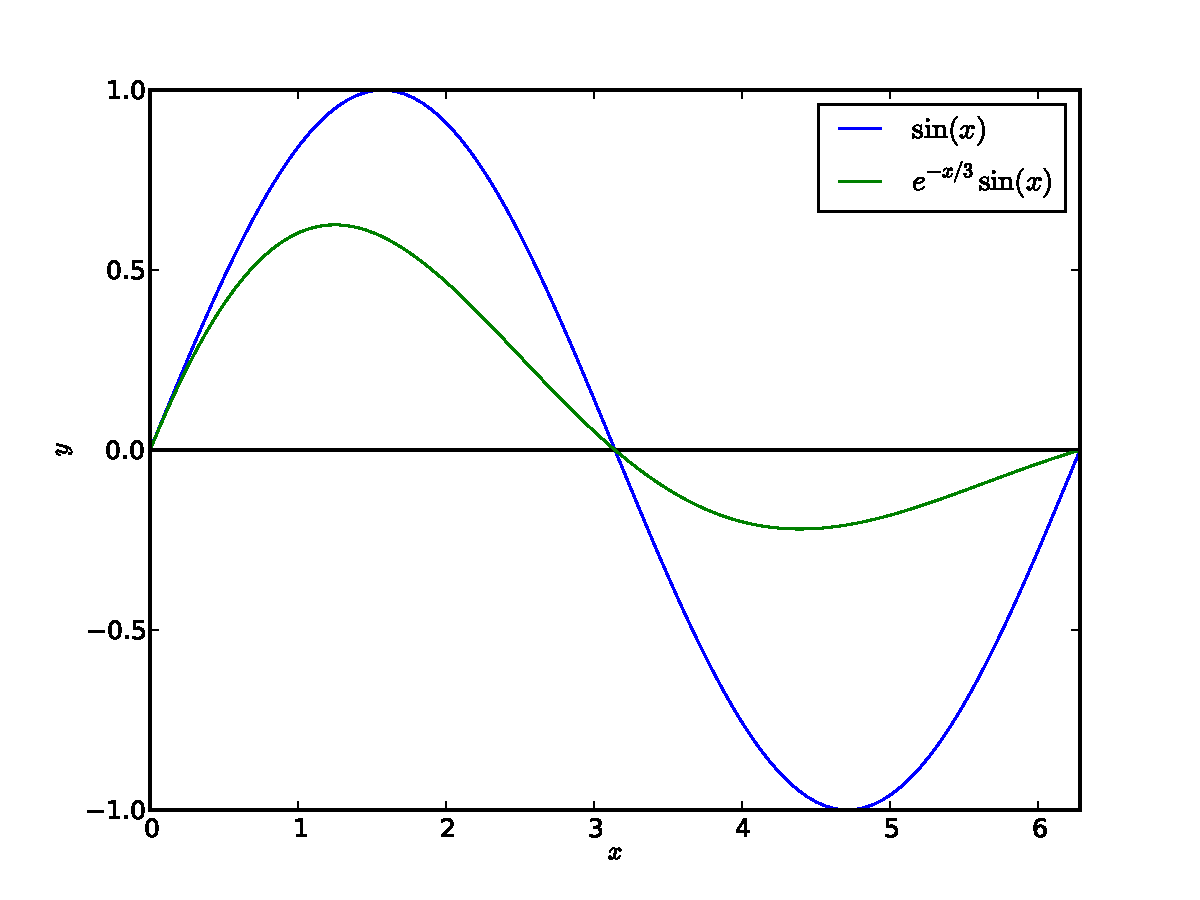
\includegraphics[height=\textwidth]{Chapter-2/figs/sine}
\caption{Delivery ratio, end-to-end delay, hops and overhead for petal routing in a spherical arrangement of UAVs.}
\label{fig:petal_spherical}
\end{figure}
\end{landscape}

\thispagestyle{lscapedplain}
\begin{landscape}
\begin{figure}
\centering
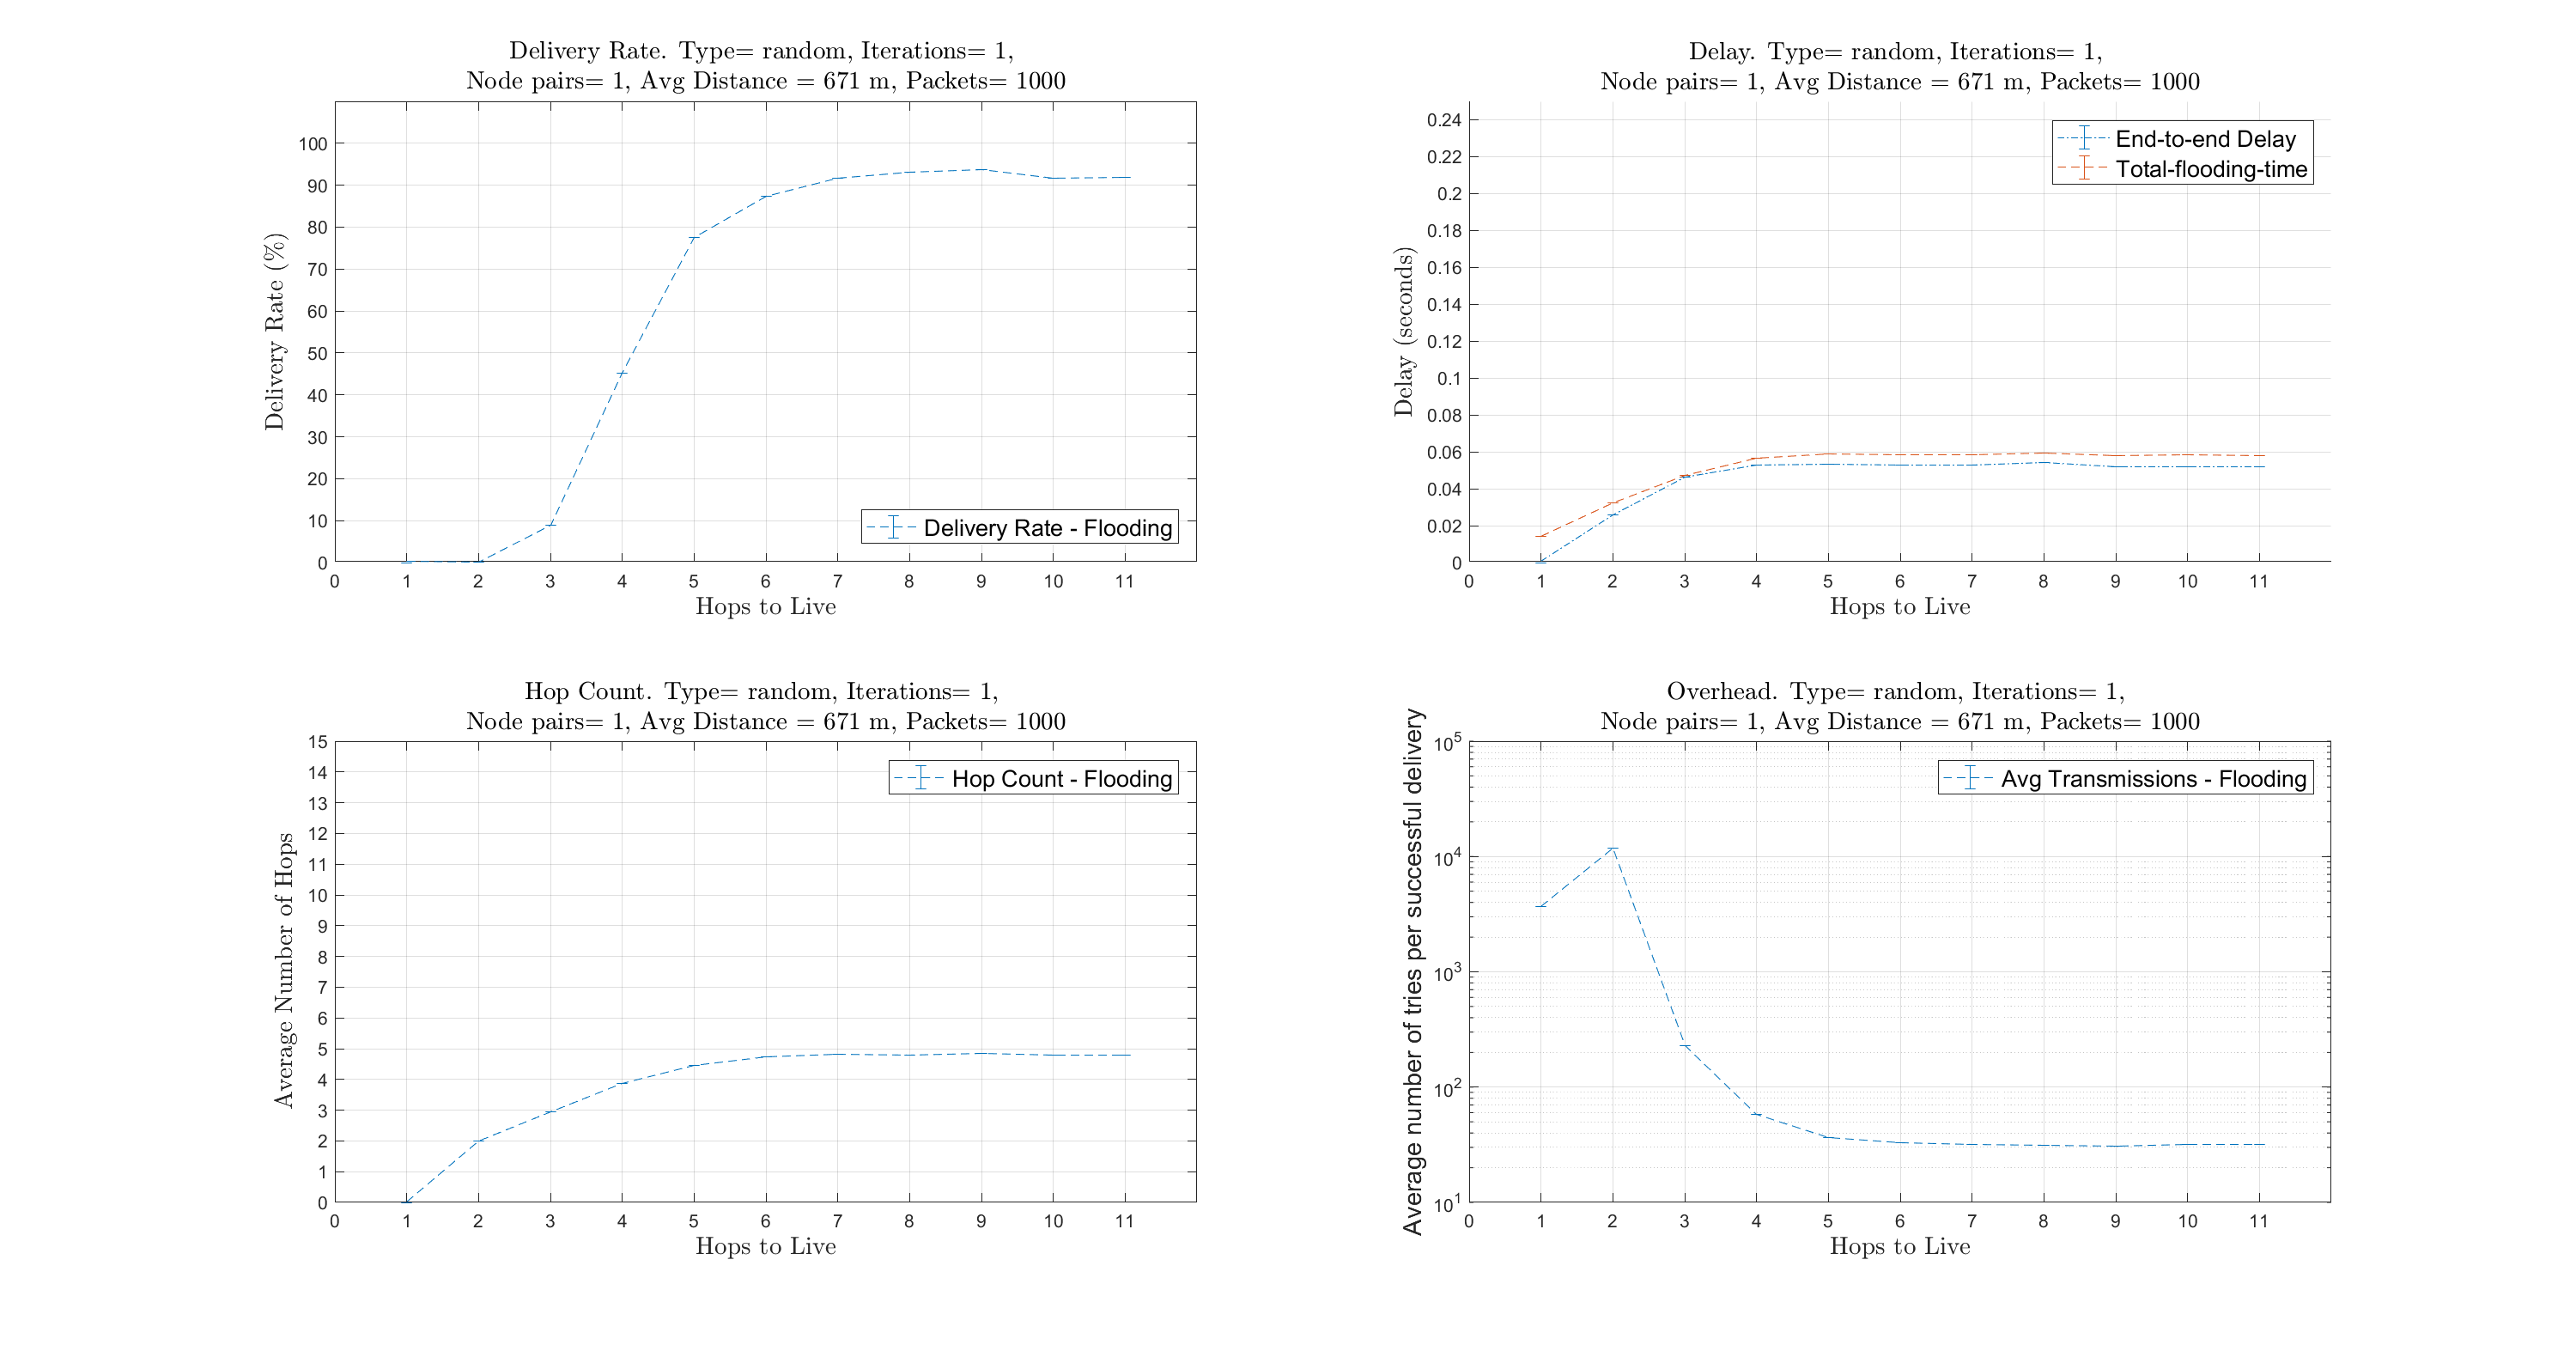
\includegraphics[width=1\textwidth]{ncsuthesis-0.6/Appendix-A/figs/flood_random.png}
\caption{Delivery ratio, end-to-end delay, hops and overhead for flooding algorithm in a random distribution of UAVs.}
\label{fig:flood_random}
\end{figure}
\end{landscape}

\thispagestyle{lscapedplain}
\begin{landscape}
\begin{figure}
\centering
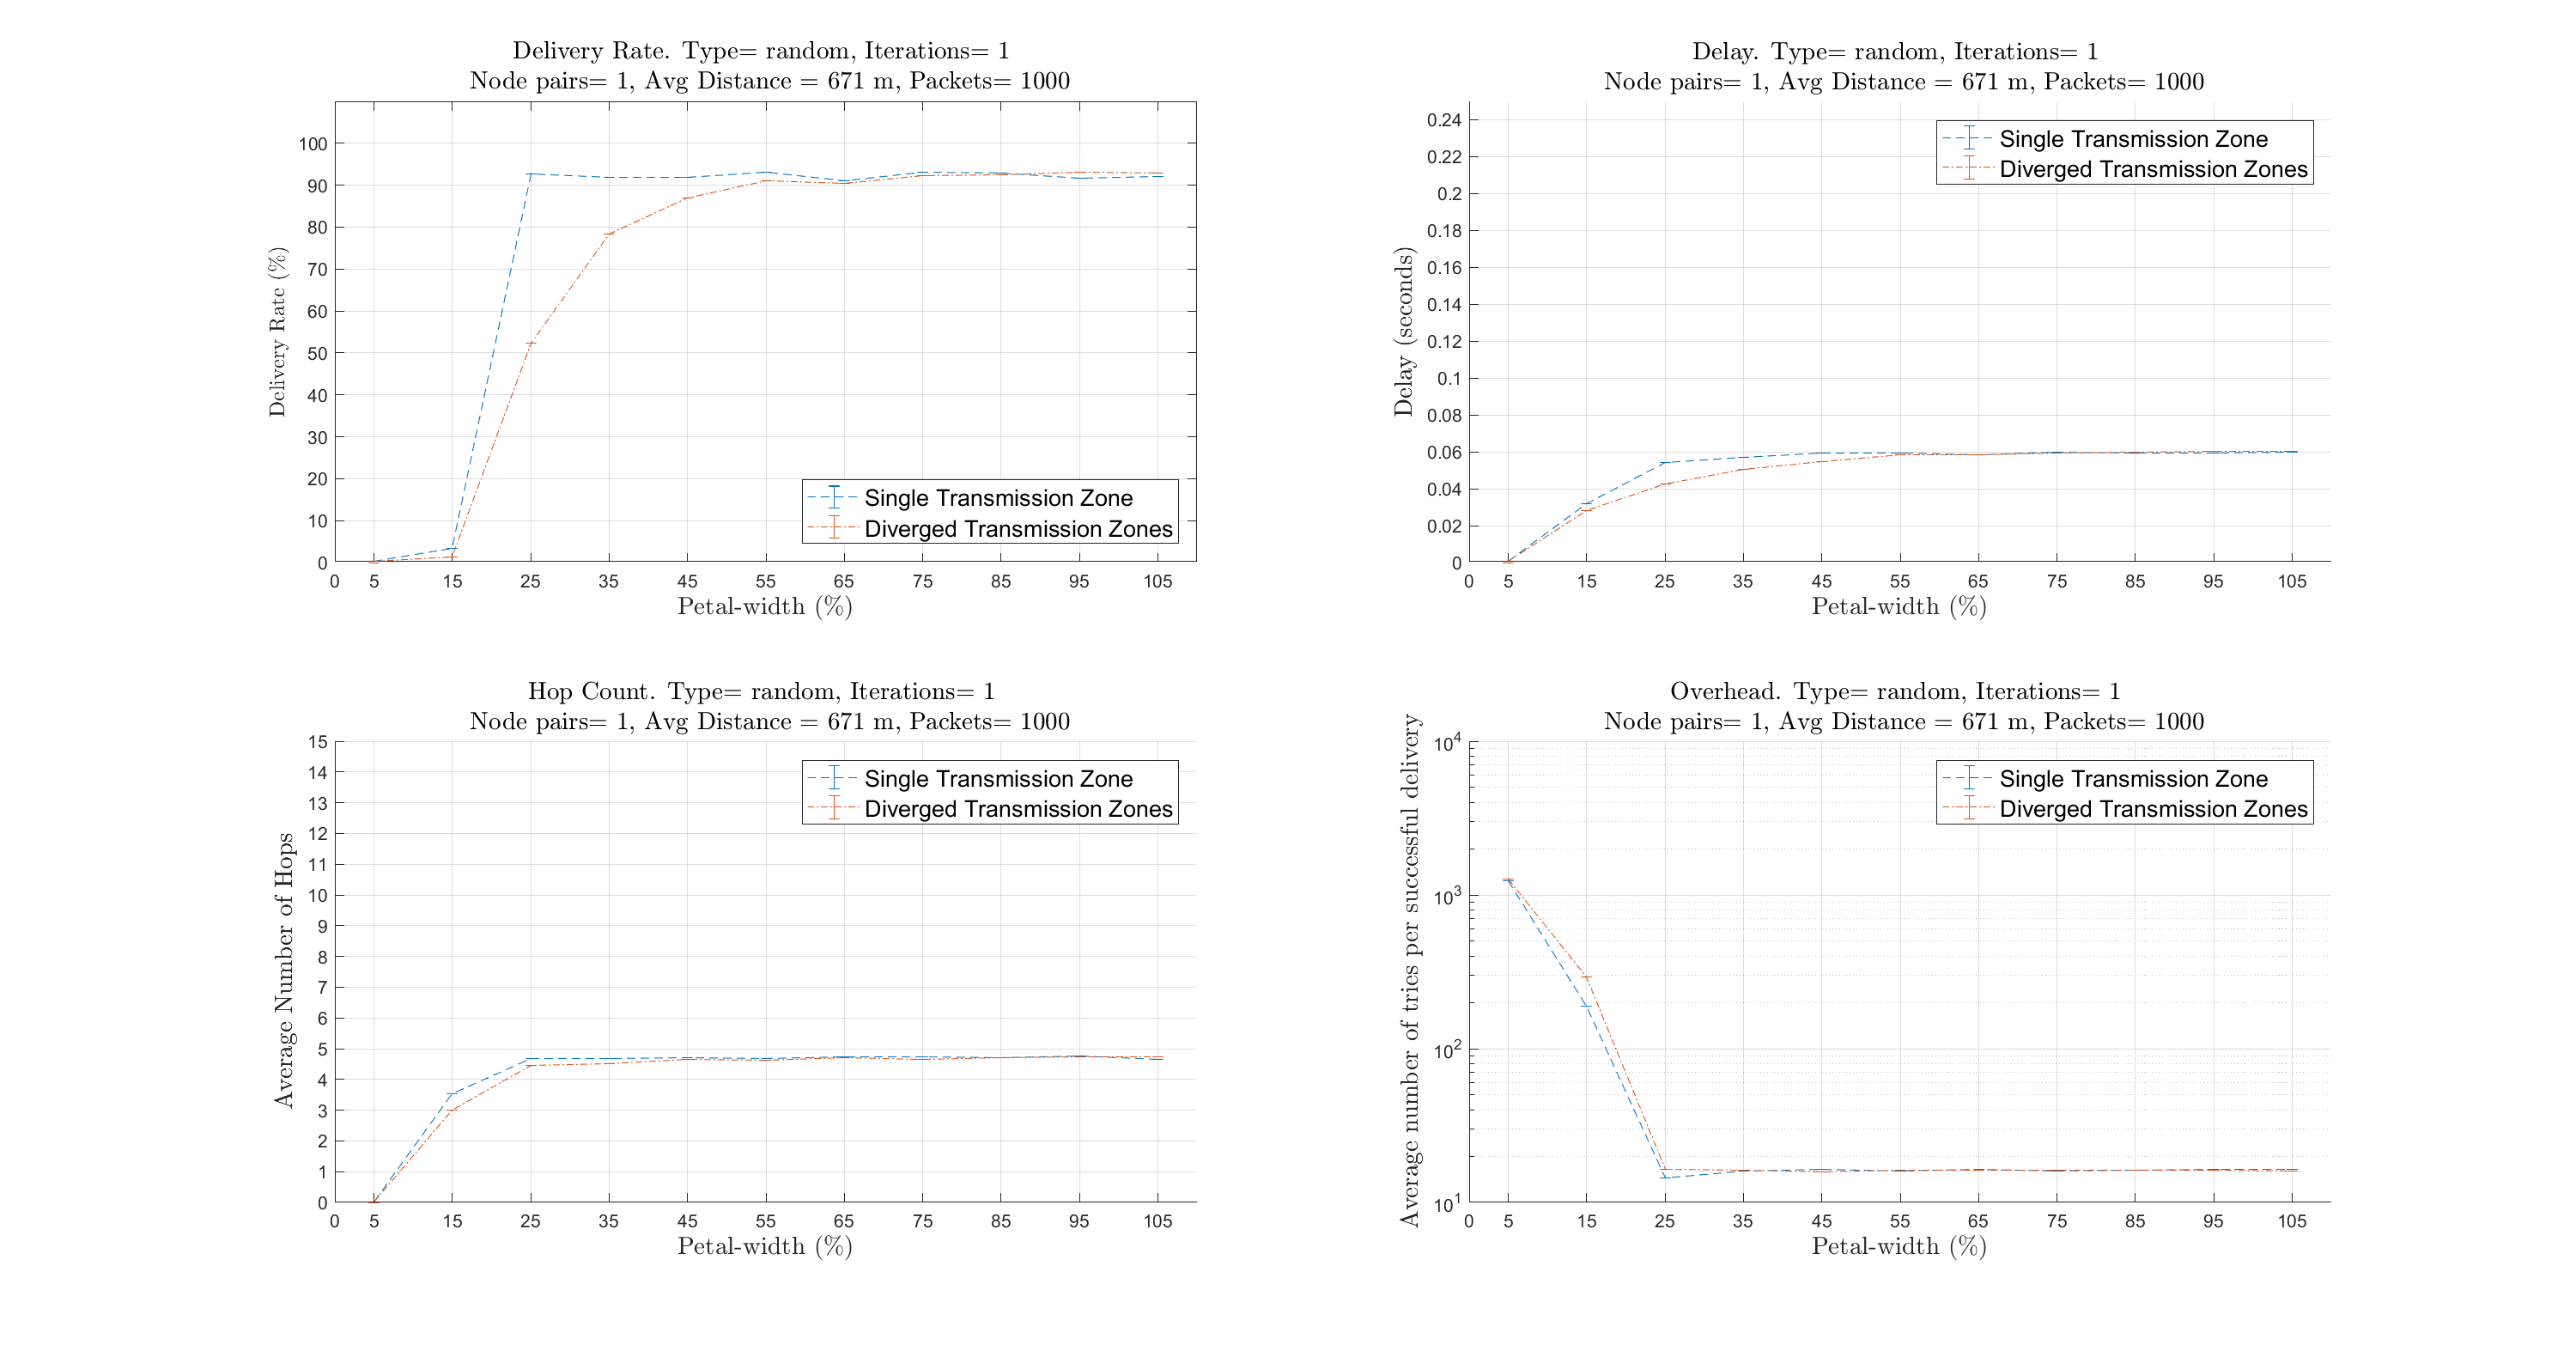
\includegraphics[width=1\textwidth]{ncsuthesis-0.6/Appendix-A/figs/petal_random.png}
\caption{Delivery ratio, end-to-end delay, hops and overhead for petal routing in a random distribution of UAVs.}
\label{fig:petal_random}
\end{figure}
\end{landscape}

\restoregeometry
\pagestyle{plain}
\thispagestyle{plain}
\newgeometry{margin=1in,lmargin=1.25in,footskip=\chapterfootskip, includehead, includefoot}



\restoregeometry

%%---------------------------------------------------------------------------%%
%\ensureoddstart
\backmatter

\end{document}
